%%
%% main.tex
%% Formatted NIP thesis conformed with the CS guidelines for the MS
%% Thesis and PhD Dissertation accepted for year 2005 onwards.
%% See nip.sty for possible modifications.
%%
%% Copyright (C) 2006  Johnrob Y. Bantang: johnrob.bantang@gmail.com
%%
%% This tex is free; you can redistribute it and/or modify it under
%% the terms of the GNU General Public License as published by the
%% Free Software Foundation version 2. See gpl.txt.
%%
%% This tex files are distributed in the hope that it will be useful,
%% but WITHOUT ANY WARRANTY; without even the implied warranty of
%% MERCHANTABILITY or FITNESS FOR A PARTICULAR PURPOSE.  See the GNU
%% General Public License for more details.
%%
%% You should have received a copy of the GNU General Public License
%% along with this program; if not, write to the Free Software
%% Foundation, Inc., 51 Franklin Street, Fifth Floor, Boston, MA
%% 02110-1301, USA.
%%
%%

\documentclass[]{nip} %%use nip class
%% to add options: phd, ms, bs, applied
%\usepackage[headsep=1in]{geometry}
\usepackage{fancyhdr}
\fancyhf{}
\rhead{\textbf{\nouppercase{\rightmark}}}
\cfoot{\thepage}

%%packages to be used.

%\usepackage[square,numbers,sort&compress]{natbib}
\usepackage[backend=bibtex,firstinits,style=numeric-comp,sorting=none, doi=false, isbn=false]{biblatex} \addbibresource{library}
   %% square-bracketed, numbered, sorted, and compressed citations
   %% for more info: http://merkel.zoneo.net/Latex/natbib.php
\usepackage{verbatim} %% for \verbatiminput
\usepackage{graphicx} %% for the graphics environment
\usepackage[centertags]{amsmath}
\usepackage{enumitem}
\usepackage{amsfonts}
\usepackage{amssymb}
\usepackage{amsthm}
%\usepackage{psfrag}
\usepackage{newlfont}
\usepackage{subfigure}
\usepackage{url}
\usepackage[labelfont=bf]{caption}
\usepackage[nameinlink, capitalize]{cleveref}
\captionsetup[figure]{width=0.9\textwidth}


\def\table{\def\figurename{Table}\figure}
\let\endtable\endfigure 
\renewcommand\listfigurename{List of Figures and Tables}


%%for appendix
\usepackage{listings}
\usepackage{textcomp}
\usepackage[usenames,dvipsnames]{xcolor}
\definecolor{listinggray}{gray}{0.9}
\definecolor{lbcolor}{rgb}{1,1,1}
\lstset{
	backgroundcolor=\color{lbcolor},
	tabsize=2,    
	%   rulecolor=,
	language=Python,
	basicstyle=\scriptsize,
	upquote=true,
	columns=fixed,
	showstringspaces=false,
	extendedchars=false,
	breaklines=true,
	prebreak = \raisebox{0ex}[0ex][0ex]{\ensuremath{\hookleftarrow}},
	frame=single,
	numbers=left,
	showtabs=false,
	showspaces=false,
	showstringspaces=false,
	identifierstyle=\ttfamily,
	keywordstyle=\color[rgb]{0,0,1},
	commentstyle=\color[rgb]{0.026,0.112,0.095},
	stringstyle=\color[rgb]{0.627,0.126,0.941},
	numberstyle=\color[rgb]{0.205, 0.142, 0.73},
	%        \lstdefinestyle{C++}{language=C++,style=numbers}’.
}
\lstset{
	backgroundcolor=\color{lbcolor},
	tabsize=2,
	language=Python,
	captionpos=b,
	tabsize=3,
	frame=lines,
	numbers=left,
	numberstyle=\tiny,
	numbersep=5pt,
	breaklines=true,
	showstringspaces=false,
	basicstyle=\footnotesize,
	%  identifierstyle=\color{magenta},
	keywordstyle=\color[rgb]{0,0,1},
	commentstyle=\color{green},
	stringstyle=\color{red}
}


\usepackage{booktabs}
\usepackage{fancyhdr}
\fancyhf{}
\rhead{\textbf{\nouppercase{\rightmark}}}
\cfoot{\thepage}

\makeatletter
\def\ignorecitefornumbering#1{%
	\begingroup
	\@fileswfalse
	#1%                     % do \cite comand
	\endgroup
}
\makeatother

%% Header section
\title{Phase-shift profilometry calibration for an artifact-free 3D reconstruction} %%required
\author{Ritz Ann Paccarangan Aguilar} %% required
\email{raguilar@nip.upd.edu.ph}%% appears only when draft version use \draft option.
\adviser{Maricor Soriano}{Ph.D.}%% required
\reader{Lean Dasallas}{M.Sc.}%% required
\secondReader{Dianne Ca\~neso}{M.Sc.}%% optional if with coadviser
%\coadviser{Another A. Adviser}{Ph.D.}%% replace "\coadviser" with "\secondReader" if no co-adviser
\director{Roland V. Sarmago}{Ph.D.}%% required
\dean{Jose Ma. P. Balmaceda}{Ph.D.} %%required
\gradyear{2015} \gradmonth{June} %%graduation month and year
\defenseDate{21 May 2015}

%% Preliminary pages' contents input here..
%\dedication{ \input{dedication.tex} }%% optional, see dedication.tex for sample content.
\acknowledgments{ \setlength{\parskip}{10pt}

College life was one great roller coaster ride with all its ups and downs. I would like to thank the following for making it fun and bearable:

My VIP family: \textbf{Prince, Peter, Ate Mabelle, Ate Angelie, Ate Lau, Kuya Francis, Ate Che, Ate Meryll, Ate Alix, Ate Badette, Kuya Gino, Kuya Aaron, Kuya Elmer, Kuya Eric, Ate Phoebe, Ate Elexis, Micholo, Jeremy,} for all the progress reports, meetings, field works, and everything we have endured together. 

\textbf{Ate Mabelle} and \textbf{Ate Angelie}, whom I talk to most frequently about random things, thank you for your advices. \textbf{Ate Phoebe}, for being my buddy in our scuba diving class. \textbf{Prince}, thank you for helping me out in my experiments during the times you were in VIP. \textbf{Peter}, I included you in VIP family for you were once a part of it but you are also a friend whom I can count on to since high school. You may have chosen a different path in college but know that I will always support you in your endeavors.

\textbf{Ate Elexis} and \textbf{Kuya Elmer}, thank you for being the best ate and kuya to me. Thank you for constantly being there when I needed help the most and for selflessly giving out the best support you can give especially during my thesis days even until the defense day. Caring for others is a natural thing for both of you and I hope that stays within you. To \textbf{Ate Elexis}, for the VIP overnights. Even if we are like cats and dogs teasing each other all the time, I know that deep inside, you have a very good heart.

\textbf{UPPA family,} thank you for being a part of my college life. Thank you for giving me a home in my first three years in college through the several \textit{tambayans} we had. You have all helped me grow as an individual.

\textbf{IPL batchmates: Julia, Alfred, Damian, Pam, Tin, Shar, Pio,} thank you for all the shared moments during our third year and fourth year, when we were in charge of all entertainments and organizing all events for IPL, respectively. Kudos to us! We did it! 

\textbf{Julia} and \textbf{Alfred}, my VIP batchmates, thank you for the countless moments we have shared from R203 to R204 to outside the corners of NIP. Thank you for the all the good and bad (if there are) times and for the laughters. To \textbf{Julia}, thank you for always finding time to listen to my stories and for your inspiring unconditional love for the people you care for. To \textbf{Alfred}, thank you for the food treats and all the good times sharing jokes and stories. Thank you as well for sharing not just your love  for physics but for music through our jamming sessions with or without guitar.

\textbf{Pam} and \textbf{Tin}, my UP Village and IPL buddies, thank you for all the stories, fun times, and academic and research stresses we have shared. To \textbf{Tin}, thank you for our get-together with \textbf{Shua} and Damian and the fun online chats even in that one year that we were housemates and our rooms were just a few feet apart, our love for online chatting still prevailed. That or we are just two people too lazy to go out of our rooms. Nah, we just love online chatting (hehe). To \textbf{Pam}, although you never reply to my hundreds of text messages, okay fine, you replied once or twice, I know that you still care. Don't worry, we now understand that me-time is a must for you once in a while.

\textbf{Jess} and \textbf{Ariel}, my food trip buddies, thank your for never failing to go out on food trips with me, together with Tin, Pam, and Damian. Never have I thought that I would be ultimate friends with the two of you in my last year of college life. Just as birds of the same feather flock together, I strongly believe that our love for food has brought us closer. \textit{Ika nga, ``Okay lang gumastos, basta sa pagkain."}

\textbf{Damian} and \textbf{Josh}, our batch is forever indebted to the two of you. Thank you for sharing all your physics, math, and computer-related skills and knowledge to us, from the very first year of college life down to the last. To \textbf{Josh}, as one who shares the same faith as mine, thank you for all our conversations which most of the time, if not always, end up in praying for one another. To \textbf{Damian}, thank you for the untiring and unfailing support you give. Thank you for always having an answer to all my academic-, research-, and even life-related questions. Thank you as well for all the corny times, honestly dude, they are the best.

To the rest of my batchmates, \textbf{Aiko, Meryll, Shami, Tom, Xavier, King, Nove, Nicole,} thank you as well for all the fun times and shared moments. Can't imagine college life without you guys. 

To those who I forgot to mention but have helped me in one way or another during my stay in college, specially in the completion of my thesis, thank you so much.

\textbf{Dr.\ Maricor Soriano}, my sincerest gratitude goes to you. Thank you for the enduring patience and for selflessly sharing your knowledge and expertise in Physics, specially in image processing. A page of this thesis is not enough if I really am to put into words and write down my gratefulness for having you as my adviser. Your love for science, not just for the sake of discovering new things, but science which you can share to the public is truly exceptional and is the ultimate thing I admire about you. 

My parents, \textbf{Ronald} and \textbf{Ruth Aguilar}, for being the best parents one can possibly have. Thank you for all the love and support - may it be moral, financial, or spiritual, and for always letting me follow my dreams. Thank you for never ceasing to pray for me. Never have I felt unloved by both of you even though we are miles apart from each other. My older brother, \textbf{Renz Aguilar}, for being protective of me and for all the times you were there when I needed help.

To the \textbf{Lord God Almighty}, all the praises, honor, and glory, I give them back to You. I am nothing without You.

%Dr.\ Ronald Banzon for the abiding jollity.

%Dr.\ Arnel Salvador, Dr.\ Armando Somintac and Dr.\ Eric Galapon for the generosity in imparting their expertise.

%The Philippine Council for Advanced Science and Technology Research and Development for the two-year financial support. The High Performance Computing Facility of the Computational Science Research Center for the permission to tap their computers.

%The Structure and Dynamics Group specially this semester's graduating students: Ms.\ Criswelynn Castro, Ms.\ Kristine Eia Antonio, Ms.\ Micielle Capili, and Ms.\ Mariel Rodriguez for remaining until the completion of our theses.

%The Papuri sa Dyos cell of the Higher Rock Christian Church specially to Ms.\ Maybelle Ninon for the persevering prayers end encouragements.

%My friends specially in the graduate school: Ms.\ Elise Stacey Agra, Ms.\ Gendith Sardane, Ms.\ Kristine Manibog, and Ms.\ Josephine Garcia for the good times. To Ms.\ Louella Judy Vasquez for the previous advices.

%Ms.\ Cyril Sadia for the unrelenting efforts in assisting and interceding.
%
%The LORD Jesus Christ who extravagantly gave all of the mentioned and unmentioned graces. } %% optional, see acknowledgment.tex for sample content.
\abstract{ A novel approach of calibrating the phase-shift profilometry (PSP) technique for an artifact-free 3D reconstruction is presented in this study. 
Artifacts caused by the fringes and the optical and digital nonlinearities of the camera-projector pair used in the PSP experiment, which include vignetting effect and inherent gamma, are carried out in the 3D reconstruction; hence, these artifacts need to be removed.  
Input-output curve of the camera-projector pair was obtained and gamma inversion was applied through nonlinear fitting of a 4th-degree polynomial function. 
Vignetting effect which causes wrong depth perception of the object was resolved through background subtraction with bicubic interpolation. 
Lastly, filtering in Fourier domain was applied to remove the unwanted sinusoidal fringe artifacts in the unwrapped phase maps. 
The artifacts were successfully removed in the 3D reconstructions of several test objects with known height/depth and replica of some characters in the Angono petroglyphs.
Depth profile analysis of the Angono petroglyphs replica was done to verify the accuracy of the measured phase-to-depth converted phase maps.
Comparison of the actual measured depths using caliper and the calibrated PSP yielded a 3.92\% error. } %% see abstract.tex
\pacs{07.05.Pj, Image processing algorithms; 42.30.Rx, Phase retrieval (optics); 33.20.Ea, Fourier transform spectra}
%\pacs{71.70.Ej (Spin-orbit coupling), 72.25-b (Spin polarized transport), 73.23-b (Electronic transport in mesoscopic systems)}

%% Main document section
\begin{document}
\maketitle %% creates title page, do not remove this line.
\makePrelim %% creates preliminary pages, do not remove this line.
\pagestyle{fancy}
\setlength{\headsep}{20pt}
\chapter{Introduction}

\section{An overview of phase-shift profilometry}
\subsection{General description}

Three-dimensional (3D) imaging techniques have a wide array of applications in medicine, manufacturing, entertainment, etc \cite{}. 
Its most common application is in the digital archiving of natural and cultural heritage sites and objects due to its non-invasive and non-contact approach \cite{Simon2013}. 

Several methods for digital 3D reconstruction have been developed for the past years. Among these methods, the structured light illumination technique, particularly phase-shift profilometry (PSP), has proven to be a simpler and cheaper yet promising method for 3D reconstruction of surfaces as compared to laser scanners and other expensive tools used in 3D imaging \cite{Zhang2002, Chrova200x}. 

PSP is a fast-acquisition 3D shape measurement measurement technique which provides high-resolution (pixel-rich) images appropriate for the study of small details in an object \cite{}. 
A PSP system consists of a projector used for projecting phase-shifted sinusoidal fringes onto the object and a camera for recording the fringe image \cite{}.

\subsection{Encountered problems in PSP}

Depending on the PSP system, an uncalibrated PSP have several artifacts which are carried out in the 3D reconstruction. 
In applications in digitization of petroglyphs in which rock art details have a very shallow depth of mostly less than 5 mm, the details are obstructed due to these artifacts, and in worst cases, they can no longer be retrieved from the resulting unwrapped phase maps.

The aforementioned artifacts arise from optical and digital nonlinearities of both the projector and camera such as vignetting effect or nonflatness of field and inherent gamma. 
Another source of artifact are the projected sinusoidal fringes which which remain in the unwrapped phase. 

Lastly, phase unwrapping method for PSP is a crucial step as it gives the absolute phase for direct conversion to actual height (depth). For typical unwrapping of phase along one dimension, noises may arise in the form of singularities which arise from undersampling of points. 

These artifacts combined greatly affect the quality of 3D reconstruction using PSP.
Hence, step by step calibration for removing these artifacts needs to be implemented in order to get the most detailed 3D reconstructions. 

\subsection{Related works}

Previous works on calibration of camera-projector pairs deal with them separately \cite{Fernandez2011}, removal of vignetting effect through per-pixel point correction\cite{Yu2004} or only for fixed camera settings \cite{Goldman}, and computing for the nonlinearity or gamma factor itself \cite{Wang2014, Baker2008}, etc. 
Such works prove to be either limited or complex methods for camera-projector pair calibration depending on the approach.

In the Philippines, as far as we know, PSP has been used twice for applications in the study and archiving of a heritage site and object. 

The first one was in 2010 wherein Vergara used PSP for the archiving of the Angono petroglyphs. 
In his thesis, he was able to reduce the artifacts introduced by the PSP system using low intensity fringe patterns to avoid the non-linear regions of the camera-projector pair and lessen the singularities by proposing a specified PSP system geometry. 

Sze’s thesis (2012) focused on phase-to-height conversion to study the graving marks of Ticao stone using PSP but was not able to address the source of branch cuts. The novelty of this research relies on the easy-to-implement algorithms for the complete removal of artifacts and branch cuts which utilizes the response curves of the camera-projector pair for non-repetitive calibration, as well as a geometry-independent and mobile PSP set-up which we can easily use for in-situ experiments.

\section{Motivations of the study}

\section{Thesis Structure}

This thesis contains 7 chapters including the Introduction in Chapter 1. An overview of PSP will be discussed in Chapter 2 which include the general algorithms used to extract phases and actual height of the objects and the setup. Chapter 3 introduces the inherent gamma of projectors and camera, how it affects the quality of the unwrapped phase maps, and the processes done to correct which involve curve fitting and interpolation. Chapter 4 proposes different background subtraction techniques for 

In this study, background subtraction with bicubic interpolation and filtering in Fourier domain were implemented in the unwrapped phase maps of a stone wall and a step pyramid to obtain an artifact-free 3D reconstruction.


%The purpose of this thesis is two-fold: (1) to deliver an analysis of parallel computing specifically on a self-constructed computer cluster; and, (2) to provide an instruction manual for other researchers so that they can set up their own affordable HPC clusters.
\chapter{3D Reconstruction using Phase-Shift Profilometry}

\section{PSP Setup}

\subsection{Schematic Diagram}
A generalized schematic setup of phase-shift profilometry is shown in Figure \ref{fig:setup}. It consists of a projector for projecting the fringes and a camera for recording. $p(x,y)$ is an arbitrary point in the object surface with a corresponding value in the image.

\captionsetup[figure]{width=5in}
\begin{figure}[h!]
	\centering
	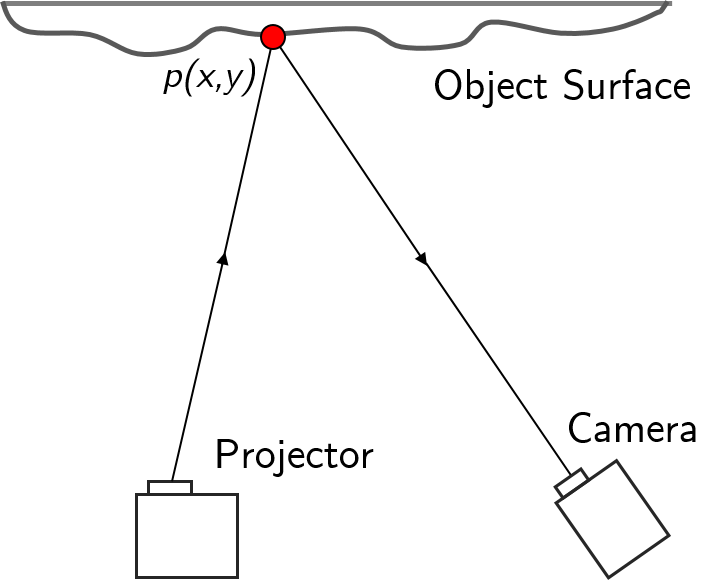
\includegraphics[width=0.475\textwidth]{figures/schematic2.jpg}
	\caption[Simplified schematic diagram of the PSP setup]{Simplified schematic diagram of the PSP setup.}
	\label{fig:setup}
\end{figure}


\subsection{Actual Setup}

An Acer DLP Projector with a resolution of 858 x 600 pixels was used to project the sinusoidal fringes to the target object and the reference in the form of a flat white board. The projected fringes were recorded by an Olympus E-500 8-megapixel DSLR Camera. 

An exposure time of 2.5 seconds for a camera aperture of f/22 was used most of the time for the camera settings. This relatively long exposure time for capturing can already be considered as ``averaging'' for reduction of noise. Images were saved as TIFF files with 3264 x 2448 pixel resolution. 

\captionsetup[figure]{width=5in}
\begin{figure}[h!]
	\centering
	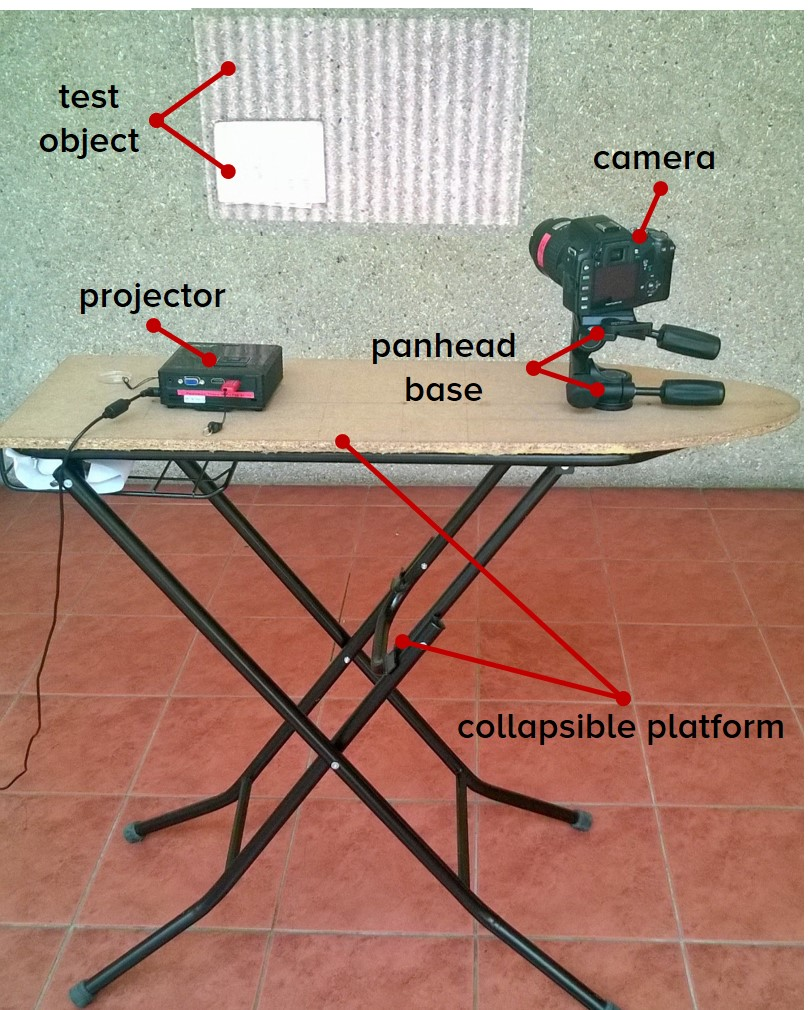
\includegraphics[width=0.42\textwidth]{figures/actualsetup.jpg}
	\caption[Actual PSP setup]{PSP experimental setup.}
	\label{fig:actual}
\end{figure}

In PSP, the stability of the setup is crucial to the output 3D reconstruction as system vibration while projecting the fringes may produce an inappropriate shift leading to error in phase computation. 

A portable mobile set-up was designed for easy-use on \textit{in-situ} experiments without sacrificing stability. The projector and camera are contained on a collapsible platform  which can be easily assembled. The camera is mounted on a panhead base for easy rotation and tilting while still maintaining its alignment with the projector. The projector is screwed on the platform to ensure that no movements will occur during fringe projection.
Shown in Figure \ref{fig:actual} is the actual setup used for PSP acquisition.

\input{PSP/flowchart.tex}
\section{Algorithm}

\subsection{Phase Wrapping}


\begin{align}
I_1(x,y)&=I_0(x,y) + I_{mod}(x,y)\cos{(\phi(x,y))}, \nonumber\\
I_2(x,y)&=I_0(x,y) + I_{mod}(x,y)\cos{(\phi(x,y)+\frac{\pi}{2})}, \nonumber\\
I_3(x,y)&=I_0(x,y) + I_{mod}(x,y)\cos{(\phi(x,y)+\pi)},\nonumber\\
I_4(x,y)&=I_0(x,y) + I_{mod}(x,y)\cos{(\phi(x,y)+\frac{3\pi}{2})},
\label{eq:four_fringes}
\end{align}  
where $I_0(x,y)$ is the average background (intensity or) grayscale value\footnote{In image processing, intensity and grayscale value are used interchangeably \cite{Gonzales}.}, $I_{mod}(x,y)$ is the grayscale value of the modulated or distorted pattern, and $I_i$, where $i=1,2,3,4$, is the grayscale value of the $i-$th image. To determine $I_0$, images of the fringe patterns projected onto a reference plane are taken. 
To determine $I_{mod}$, images of the fringe projected object are taken. 
The phase difference, which is related to the grayscale values of the images reflecting back from the distortions of the patterns along the surface height, is given by
\begin{equation}
\phi(x,y)=\tan^{-1}{\left( \frac{I_4(x,y) - I_2(x,y)}{I_1(x,y)- I_3(x,y)}\right)}
\label{eq:phase}
\end{equation}
To show Eq.~(\ref{eq:phase}), expressions in Eq.~(\ref{eq:four_fringes}) are rewritten as 
\begin{align}
I_1(x,y)=I_0(x,y) + I_{mod}(x,y)\cos{(\phi(x,y))}, \nonumber\\
I_2(x,y)=I_0(x,y) - I_{mod}(x,y)\sin{(\phi(x,y))}, \nonumber\\
I_3(x,y)=I_0(x,y) - I_{mod}(x,y)\cos{(\phi(x,y))},\nonumber\\
I_4(x,y)=I_0(x,y) + I_{mod}(x,y)\sin{(\phi(x,y))}.
\label{eq:four_fringes2}
\end{align}  
Subtracting $I_2$ from $I_4$ and $I_3$ from $I_1$ yields
\begin{align}
I_4(x,y)-I_2(x,y)&=2I_{mod}\sin{(\phi(x,y))}, \nonumber\\
I_1(x,y)-I_3(x,y)&=2I_{mod}\cos{(\phi(x,y))}.
\end{align}  
Dividing the first expression by the second, we get
\begin{equation}
\tan(\phi(x,y))=\frac{I_4-I_2}{I_1-I_3}.
\label{eq:tan_phase}
\end{equation}
Getting the inverse of Eq.~(\ref{eq:tan_phase}) results in Eq.~(\ref{eq:phase}).  The discontinuities of the tangent inverse function at $2\pi$ are removed by adding or subtracting multiples of $2\pi$.  This step is known as phase unwrapping. 

\subsection{Phase Unwrapping}

\input{PSP/testobjects.tex}

\chapter{Gamma inversion through nonlinear fitting}


\section{Inherent Gamma of camera and projectors}


GAMMA DEFINITION

Cameras have inherent gamma which changes the appearance of a digital image. This is caused by image compression on the way files are saved (JPG, TIFF, etc.) while LCD projectors do gamma correction by displaying images with adjusted pixel intensities for more detailed and enhanced projected images \cite{gamma_correction}. 


These nonlinearities combined greatly affect the quality of 3D reconstruction using PSP.


\section{Calibration through curve fitting and nonlinear interpolation}

A calibration chart of 256 gray level patches (8-bit) was projected into a flat screen to clearly demonstrate the effects of the inherent gamma of the camera-projector pair in the resulting output image. 
The pixel values from the calibration chart's output image are obtained and compared to the actual values of that of the input. 
The input vs. output (I/O) curve of the camera-projector pair was then derived.
 
From the mean of the subpixels (15x15 pixels) of each cell in the calibration chart, the values for each channel (RGB and grayscale) were plotted as seen in Figure \ref{fig:calib}. It can be observed that the camera-
projector pair has a nonlinear (S-shaped) response curve. A polynomial function of the form
\begin{equation}
y = p_1x^4 + p_2x^3 + p_3x^2 + p_4x + p_5,
\label{eq:poly}
\end{equation}
where $p_n (n = 1...5)$ are the parameters for the fitting function, was fitted to the input-output (I/O) curve of the camera-projector pair as observed in Figure \ref{fig:IO_fit}b. 

\captionsetup[figure]{width=5in}
\begin{figure}[h!t]
	\centering
	\subfigure[]{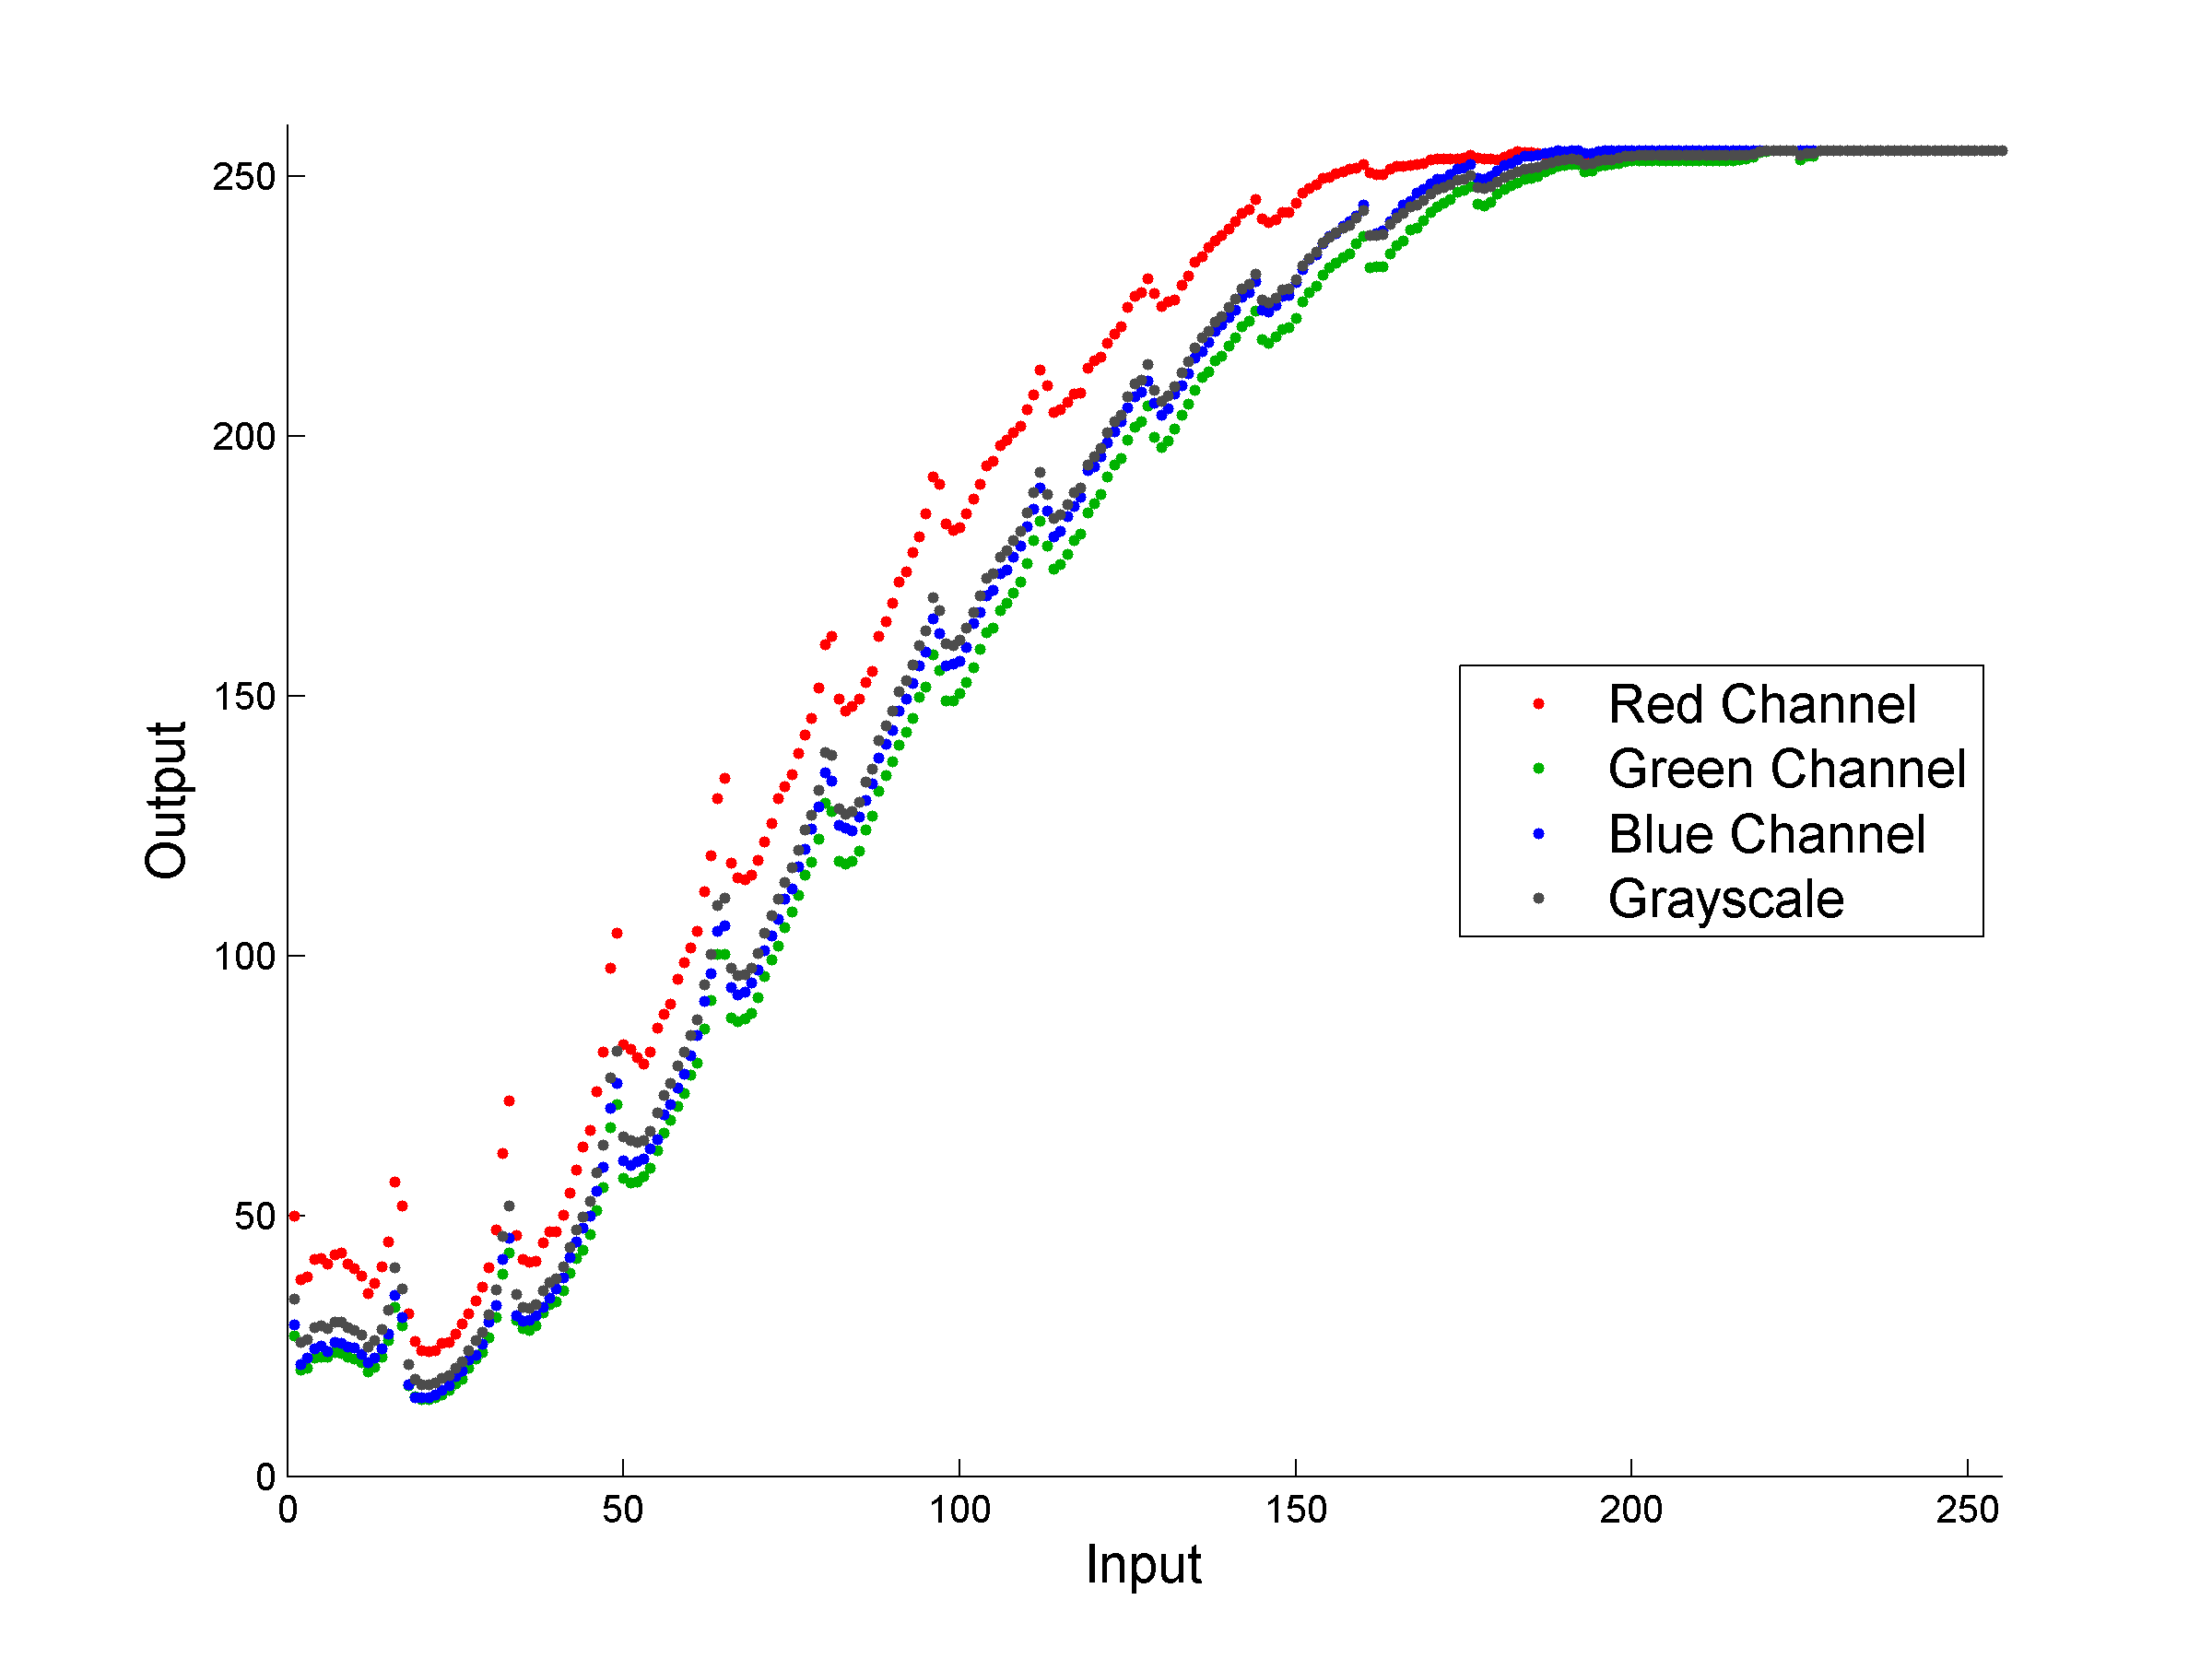
\includegraphics[width=0.475\textwidth]{figures/IOcurve_.png}\label{fig:IO}}
	\subfigure[]{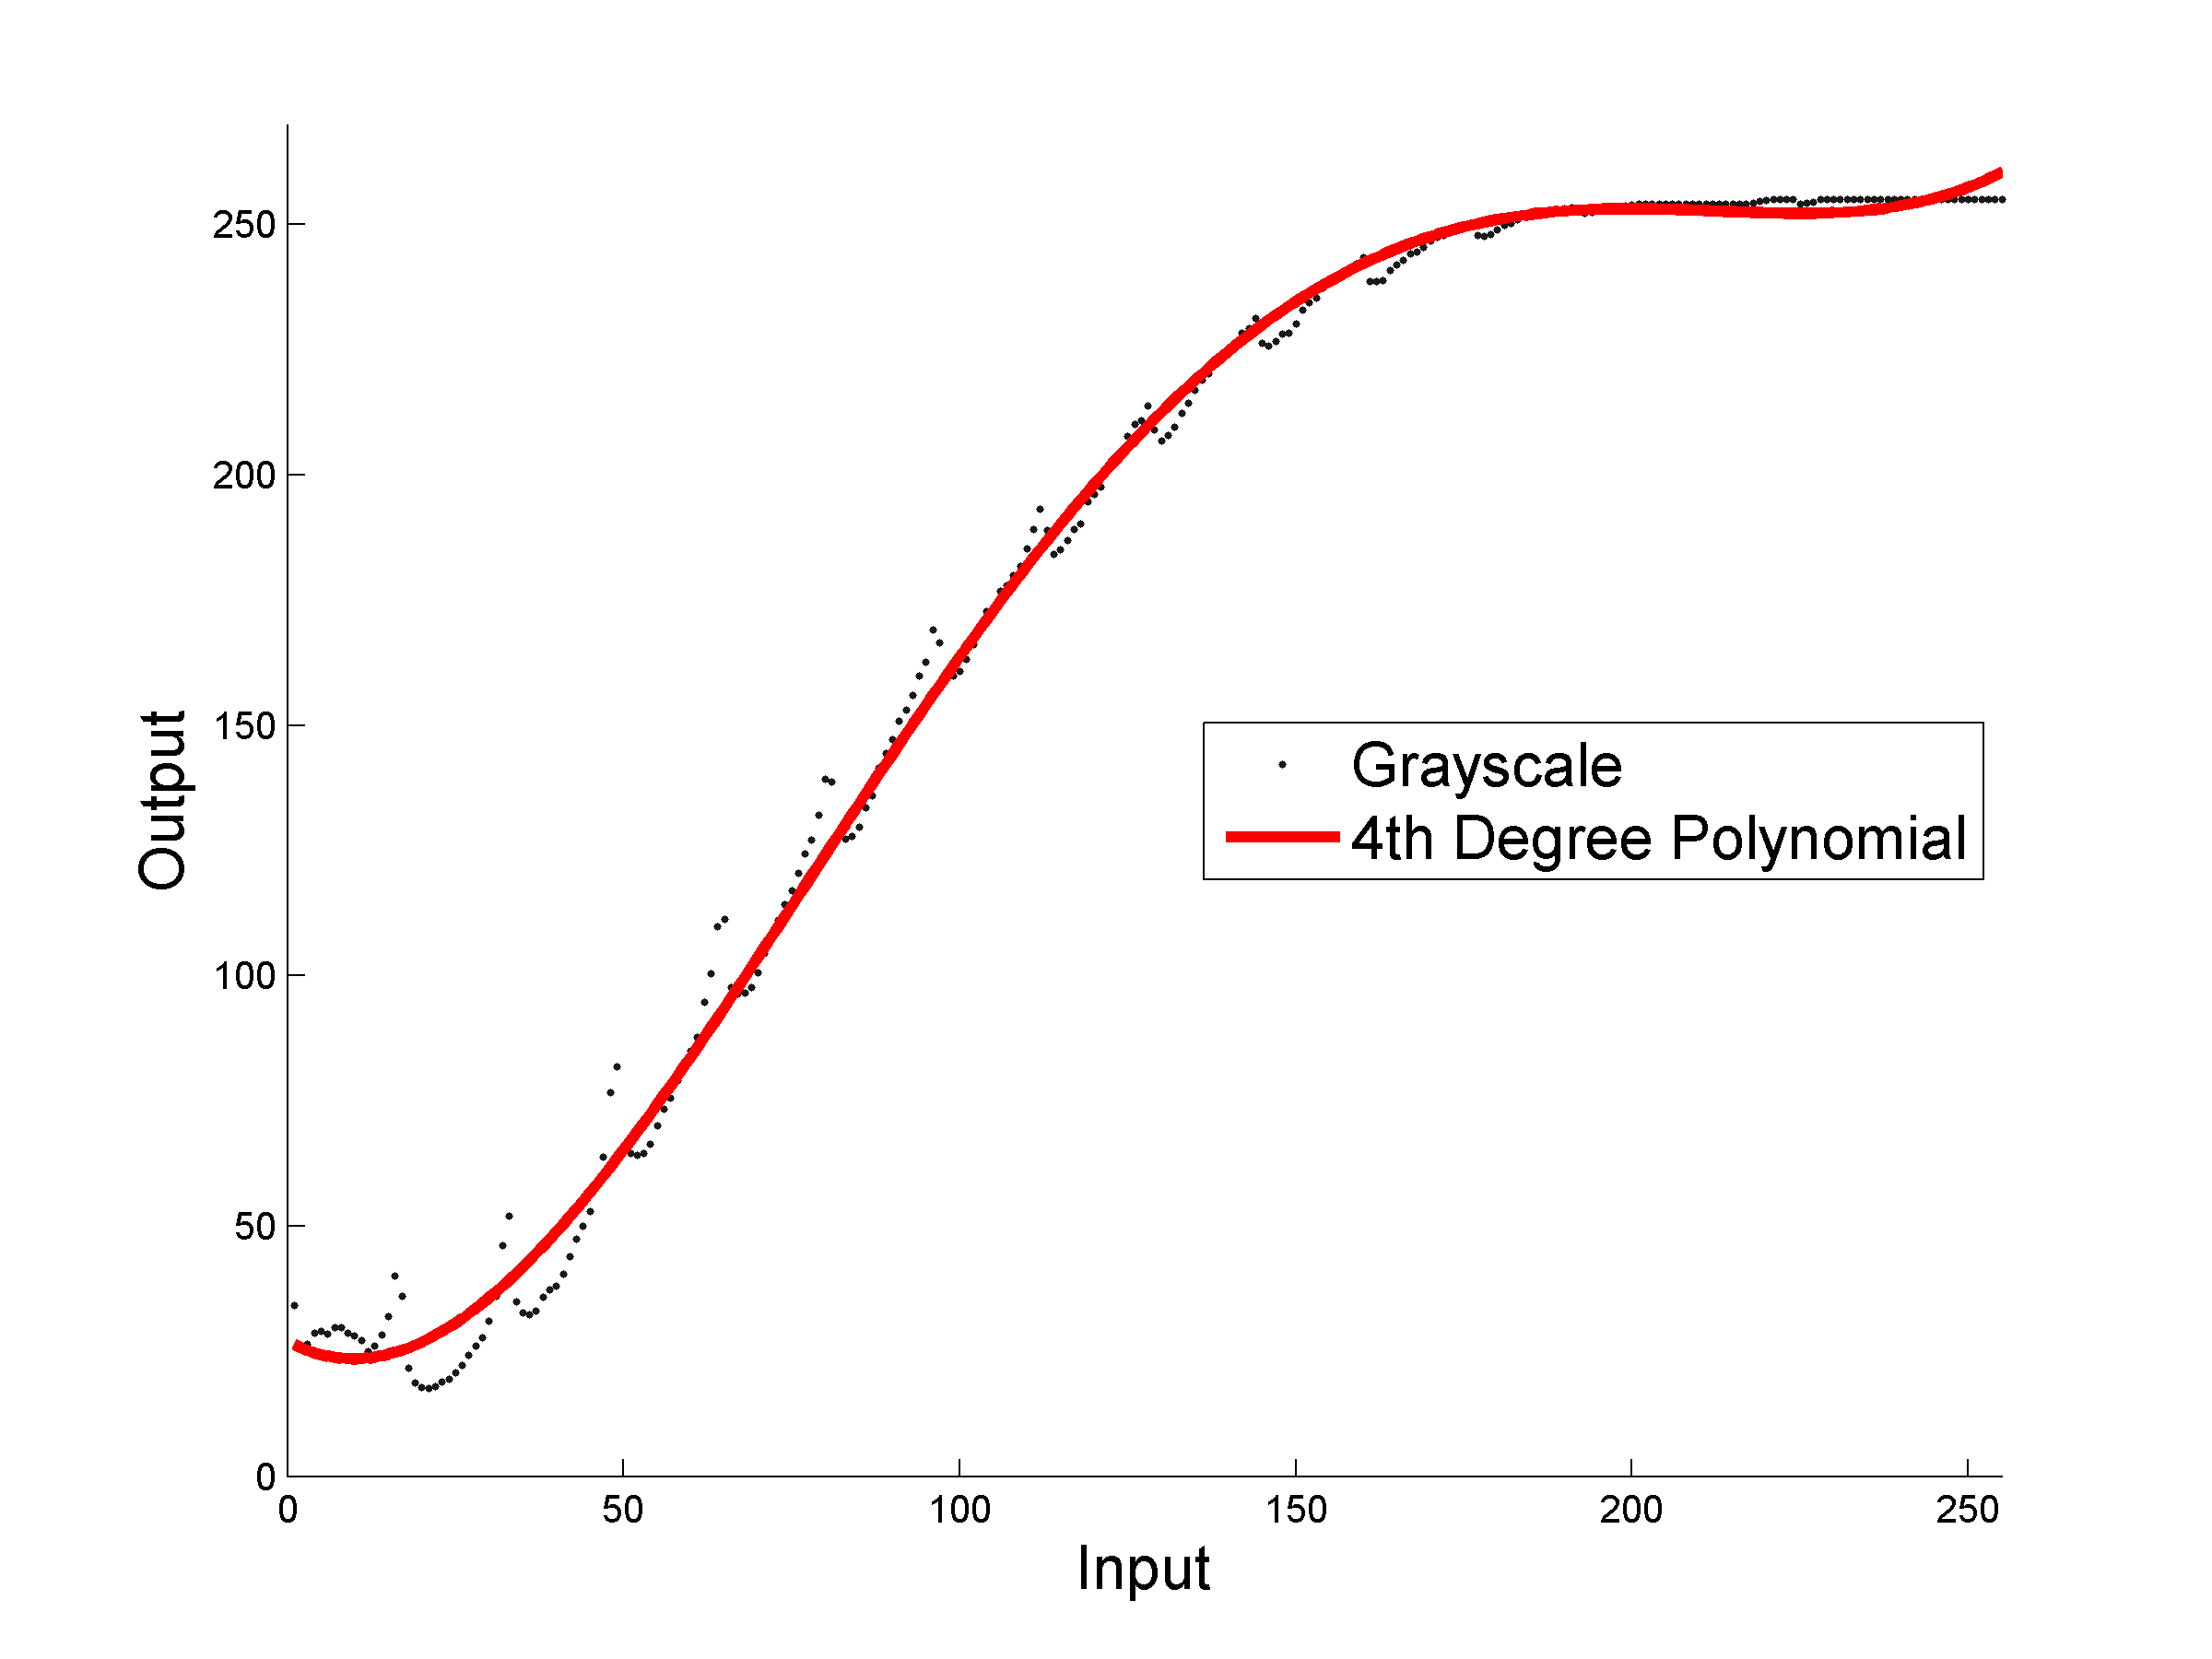
\includegraphics[width=0.475\textwidth]{figures/fits.png}\label{fig:fit}}
	\caption{\subref{fig:IO} I/O curve of the grayscale and RGB channels of each pixel value in the calibration chart and (b) the 4th degree polynomial function fitted to the grayscale using nonlinear fitting.}
	\label{fig:IO_fit}
\end{figure}



The 4th degree polynomial function served as the basis for nonlinear fitting since it gives the least number of residuals among the high-order polynomial functions. 
By knowing the actual input (0 to 255) and the polynomial function with the correct parameters, the inverse function was finally obtained via interpolation.
\captionsetup[figure]{width=5in}
\begin{figure}[h!t]
	\centering
	\subfigure[]{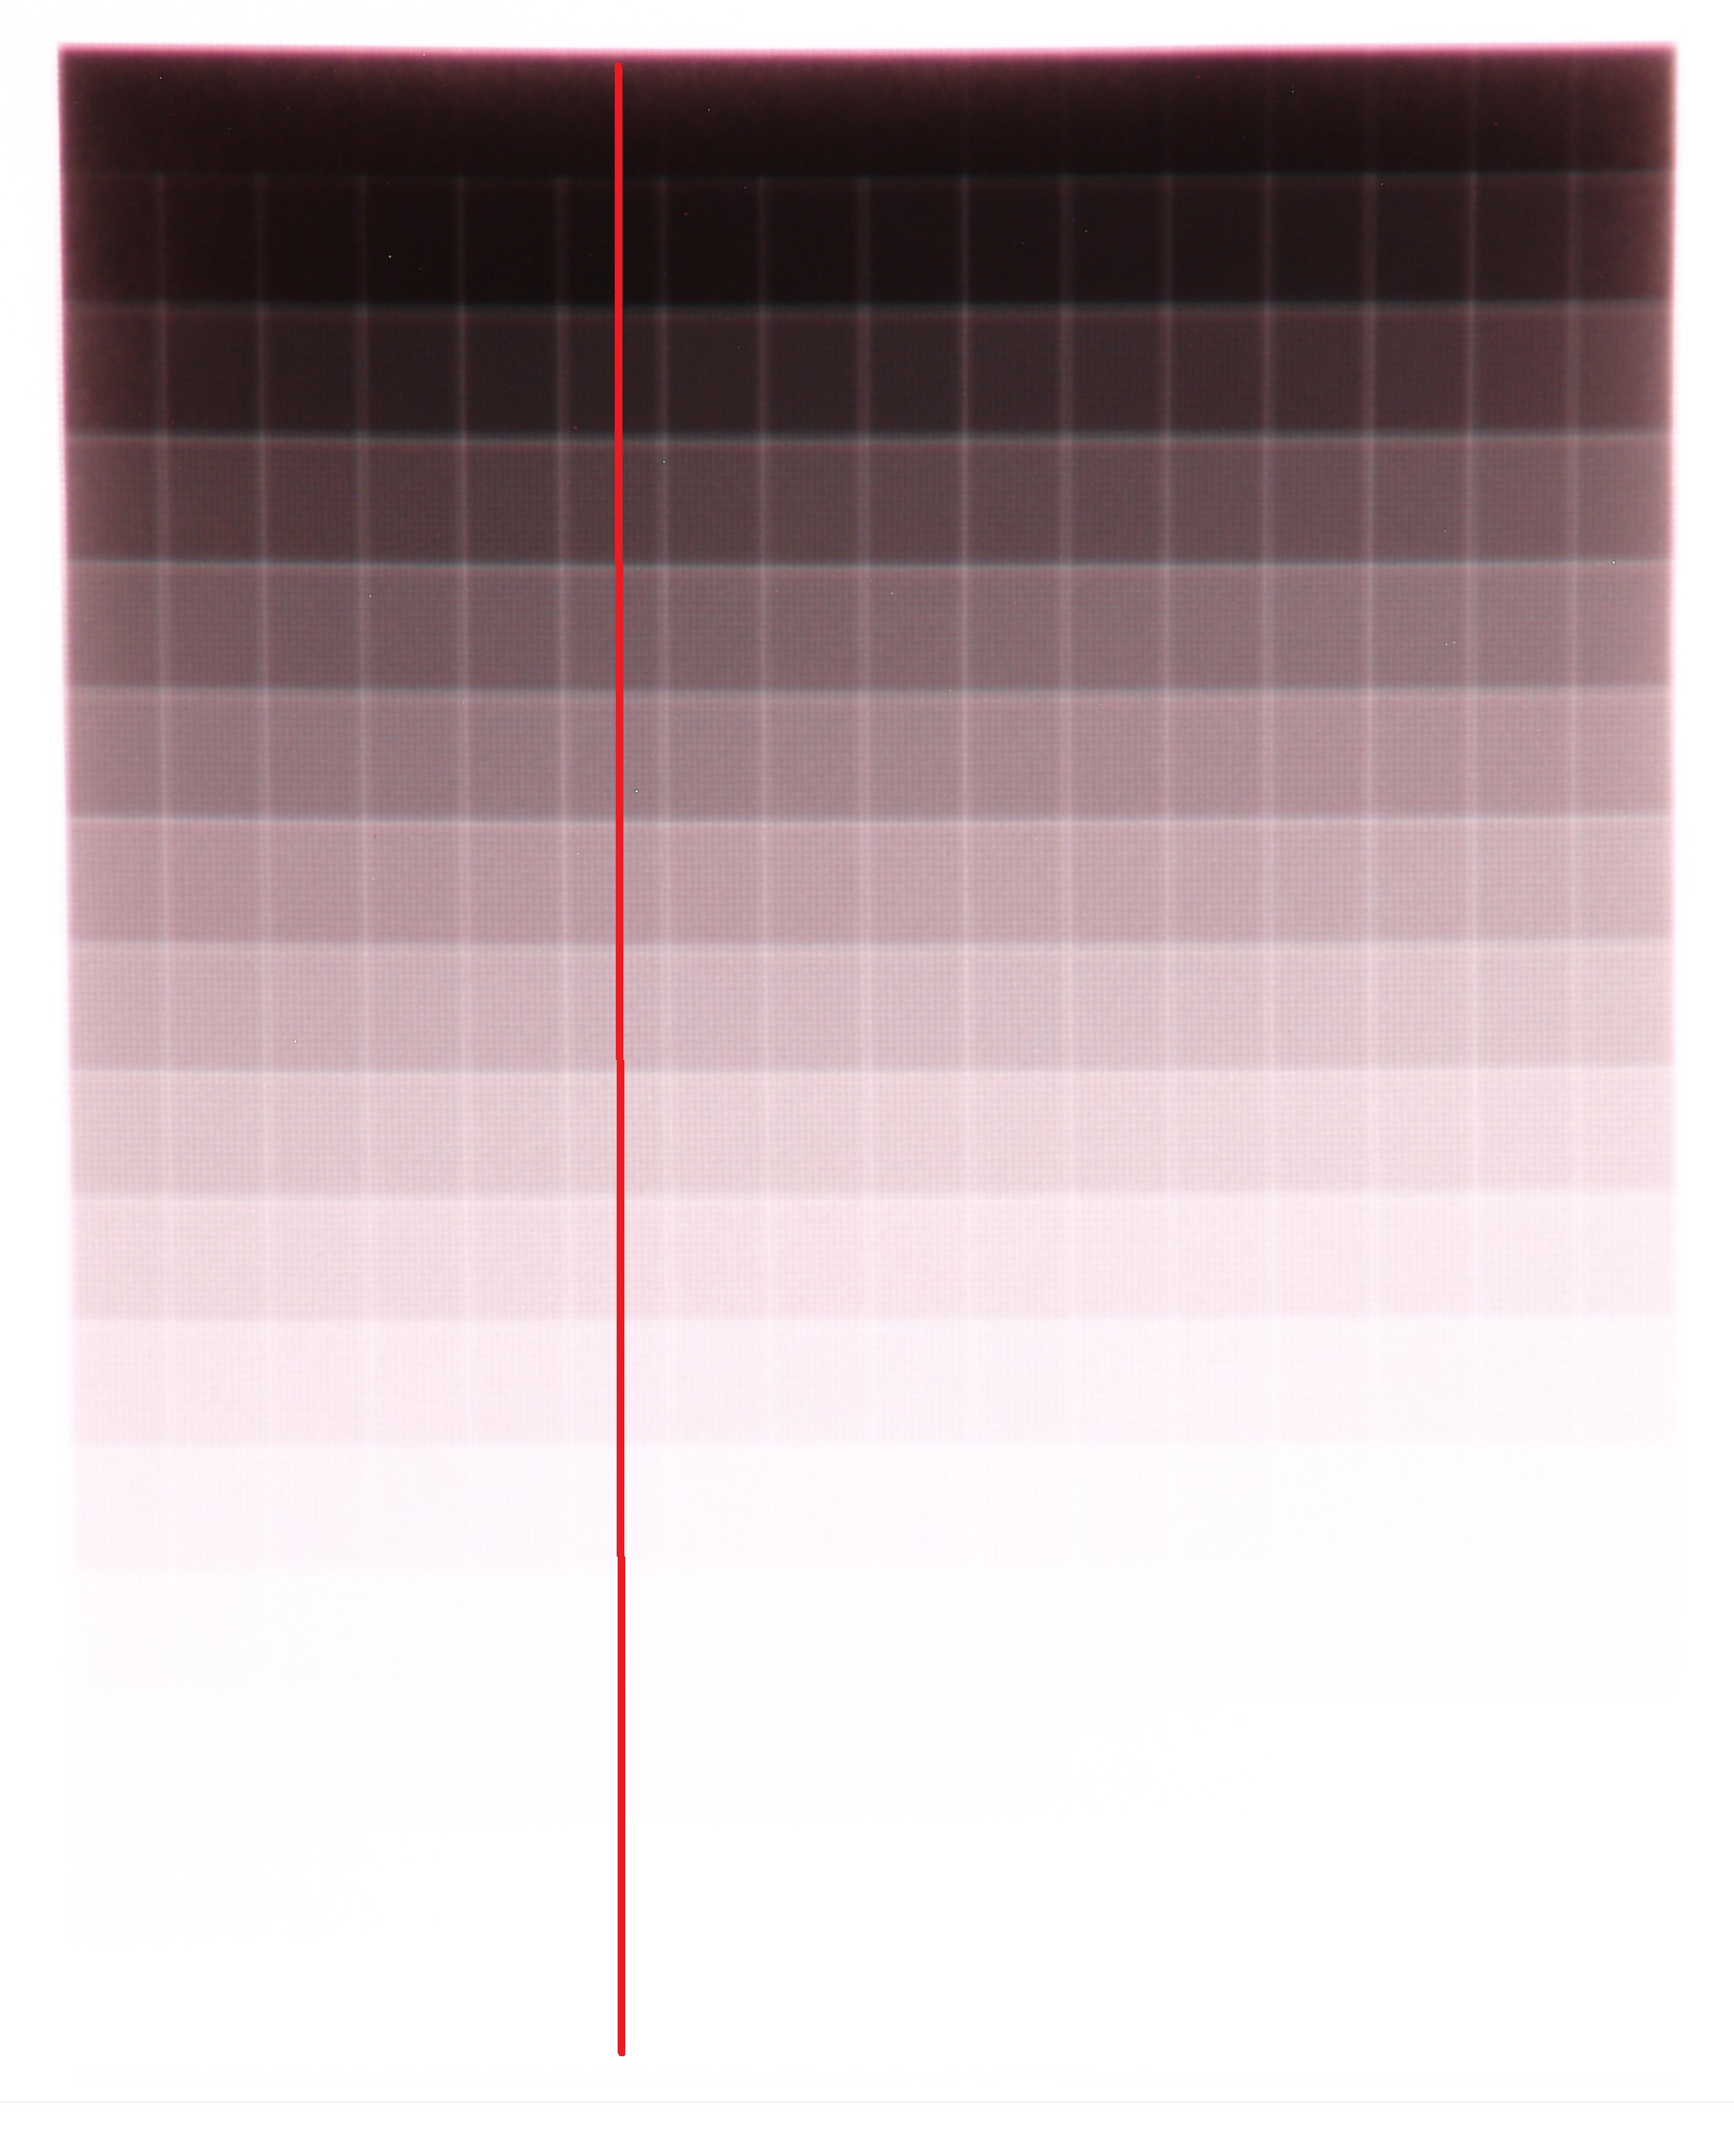
\includegraphics[height=0.35\textwidth]{figures/grid.jpg}\label{fig:input_calib}}
	\subfigure[]{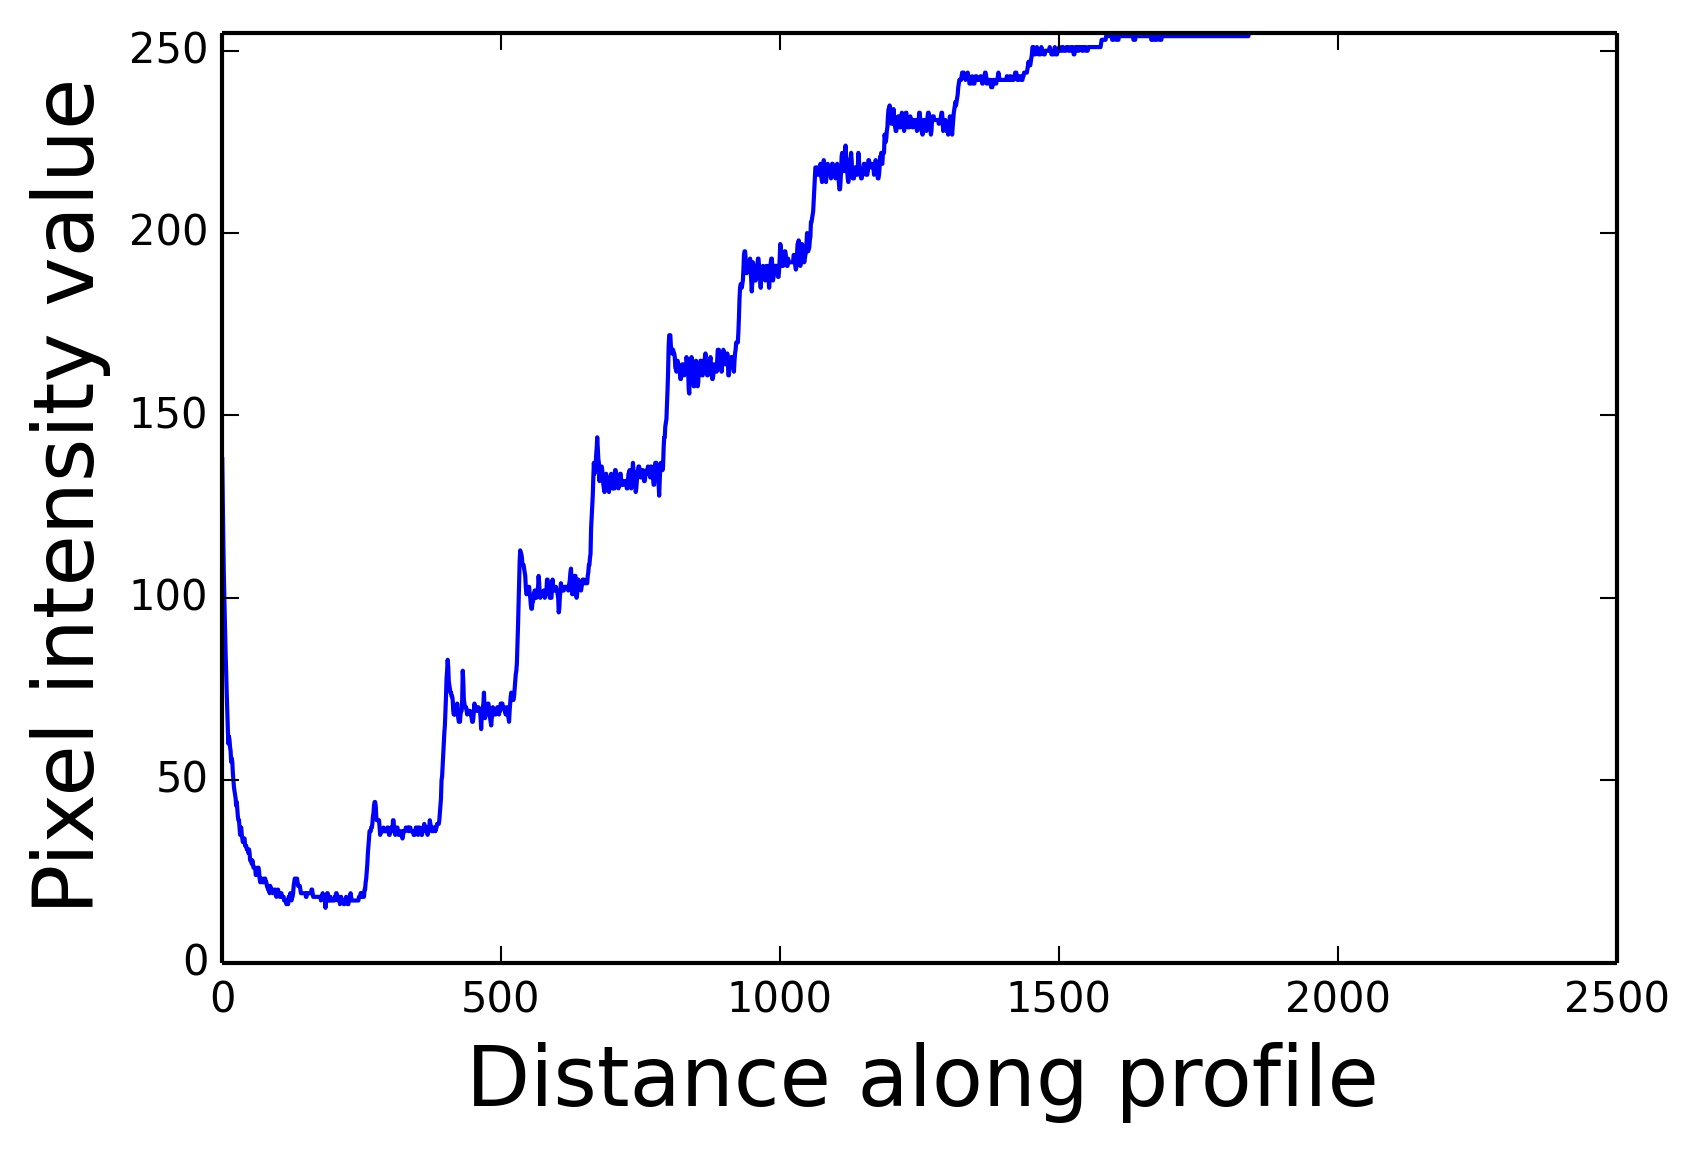
\includegraphics[height=0.35\textwidth]{figures/g_profile.jpg}\label{fig:input_profile}}
	\subfigure[]{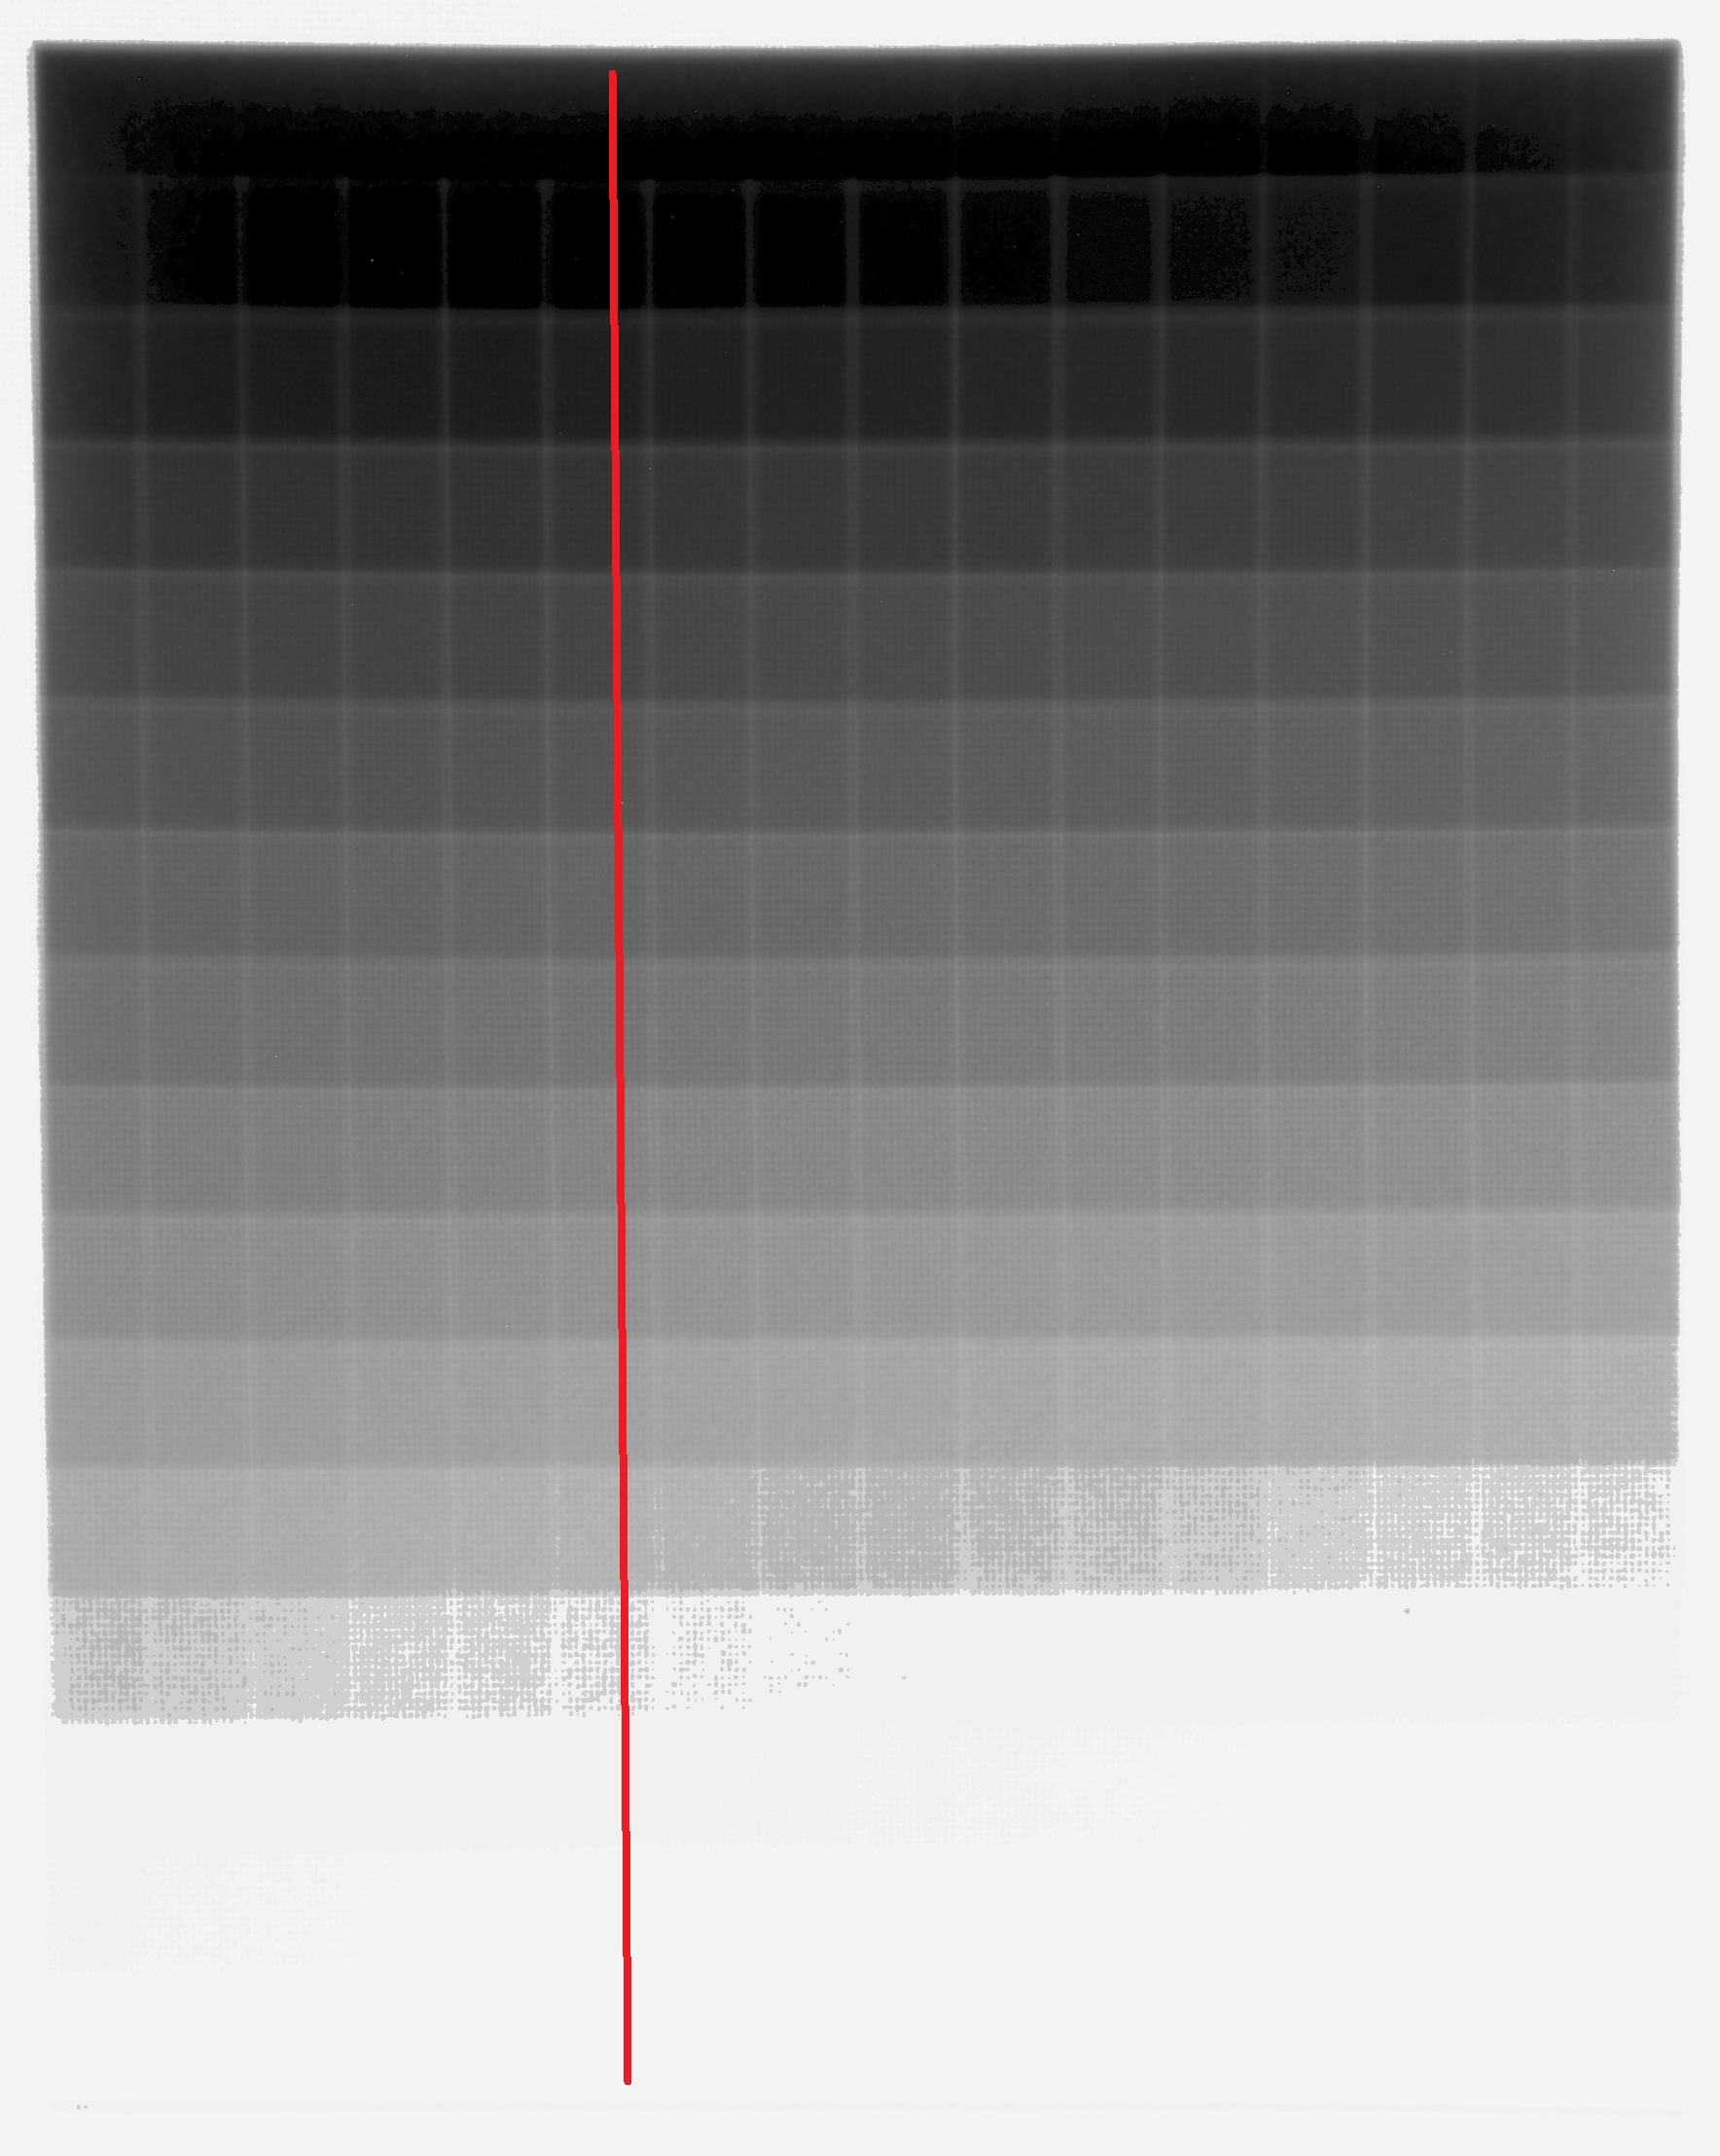
\includegraphics[height=0.35\textwidth]{figures/linear.jpg}\label{fig:linear_calib}}
	\subfigure[]{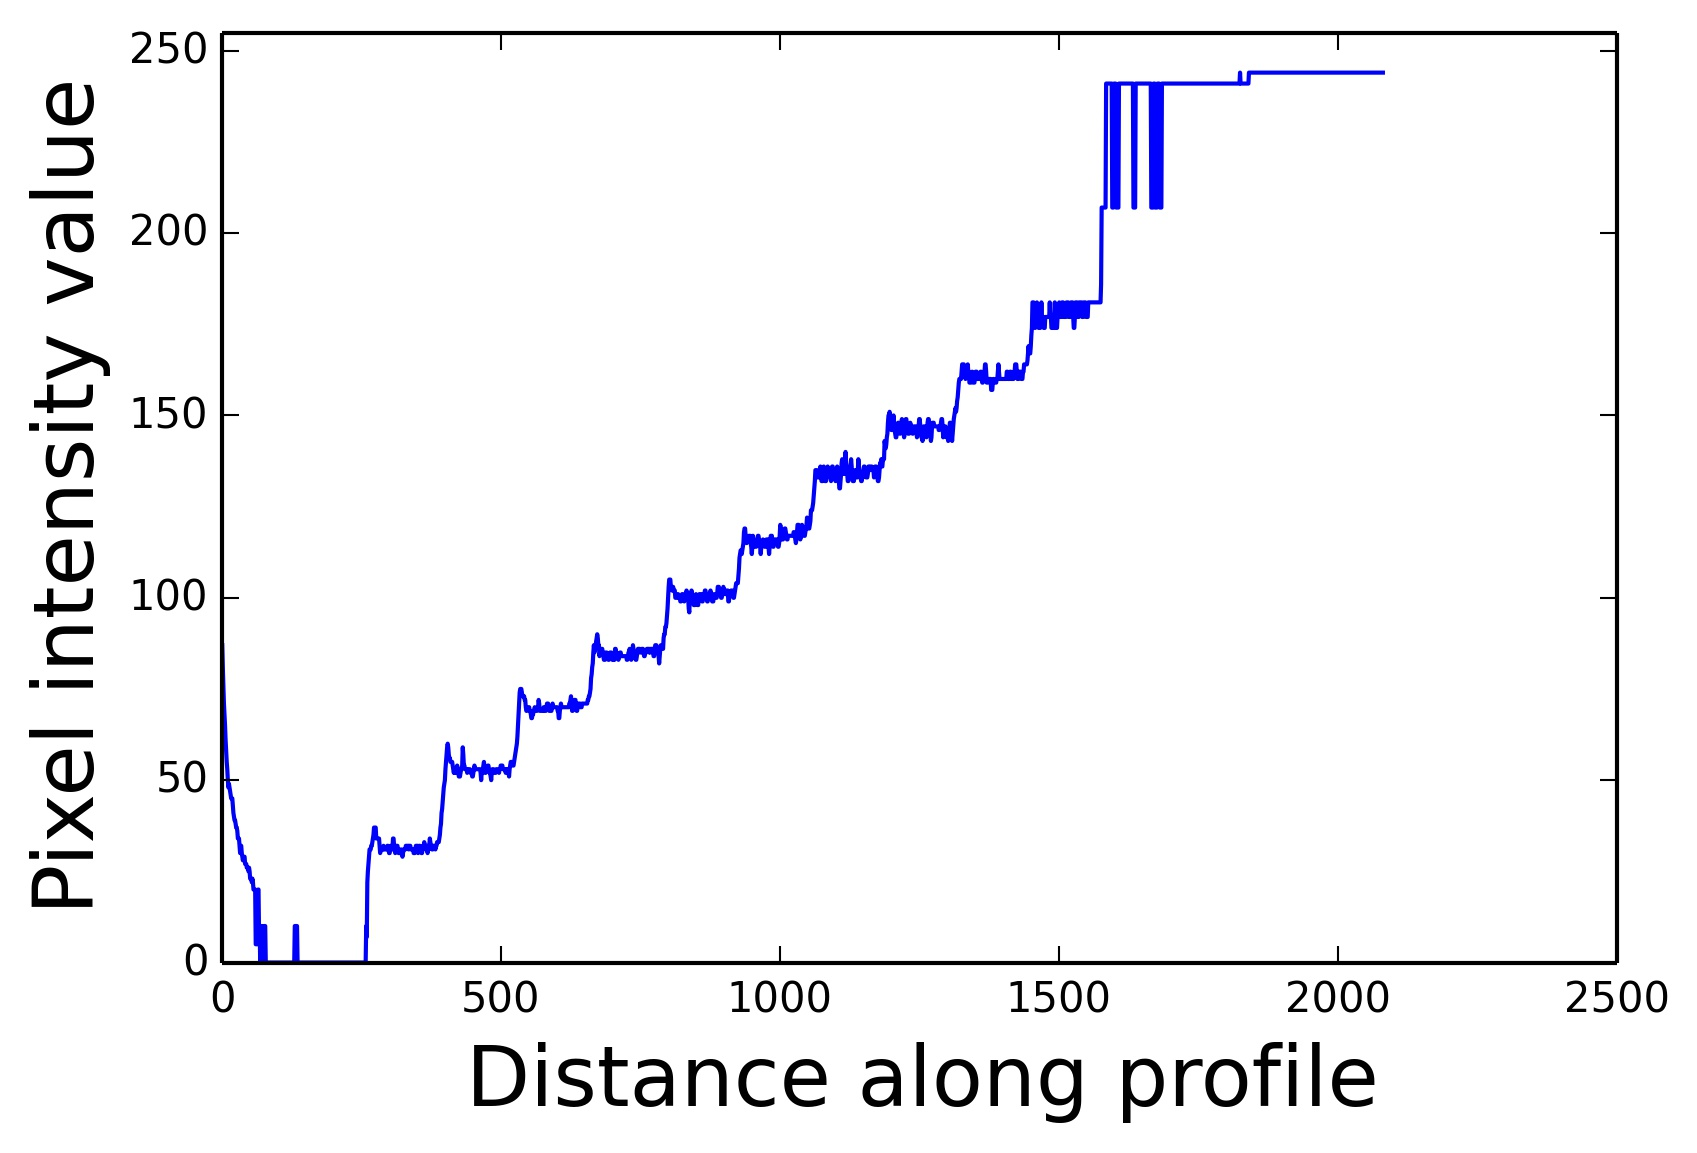
\includegraphics[height=0.35\textwidth]{figures/l_profile.jpg}\label{fig:linear_profile}}
	\caption{Calibration charts and intensity profiles (red lines): \subref{fig:input_calib} Output image and
		\subref{fig:input_profile} its intensity profile
		\subref{fig:linear_calib} Linearized output image and 
		\subref{fig:linear_profile} its intensity profile}
	\label{fig:calib}
\end{figure}

Intensity profiles of the nonlinearized and linearized output images of the calibration chart were taken to verify the effect of the linearization. 

From Figure \ref{fig:calib}, the difference in the intensity profiles are indeed visible as that of the output image takes the form of the S-shaped curve. Upon linearization, it was observed that the most linearized parts of the ouput image are the pixel values greater than 50 and less than 200, based from the intensity profile in Figure \ref{fig:calib}d. 

We notice that the high-intensity values are obscured in the linearized calibration chart (see Fig. \ref{fig:calib}c). This is due to the camera setting used wherein the exposure time of 2.5 s resulted to a high level of intensity of the overall image or a saturation, making these values hard to linearize. The high-intensity values of the linearized calibration chart had a noisy data. 

\section{Gamma inversion application in fringe biasing}
Projected fringes were initially created using a sinusoidal wave along the y-direction having the following equation:
\begin{equation}
\textrm{fringe} = I_o(\sin(2\pi f t + n\phi))
\label{sine wave}
\end{equation}
where $I_o$ is the relative intensity of the fringe set to 0.3, $f$ is the frequency set to 40 Hz, $t$ is time in seconds, $n$ is the fringe number (1 to 4), and $\phi$ is the phase shift which was set to $\pi/2$ or 90$^o$ resulting to four fringes with phase shifts of 0$^o$, 90$^o$, 180$^o$, and 270$^o$.

\captionsetup[figure]{width=5in}
\begin{figure}[h!]
	\centering
	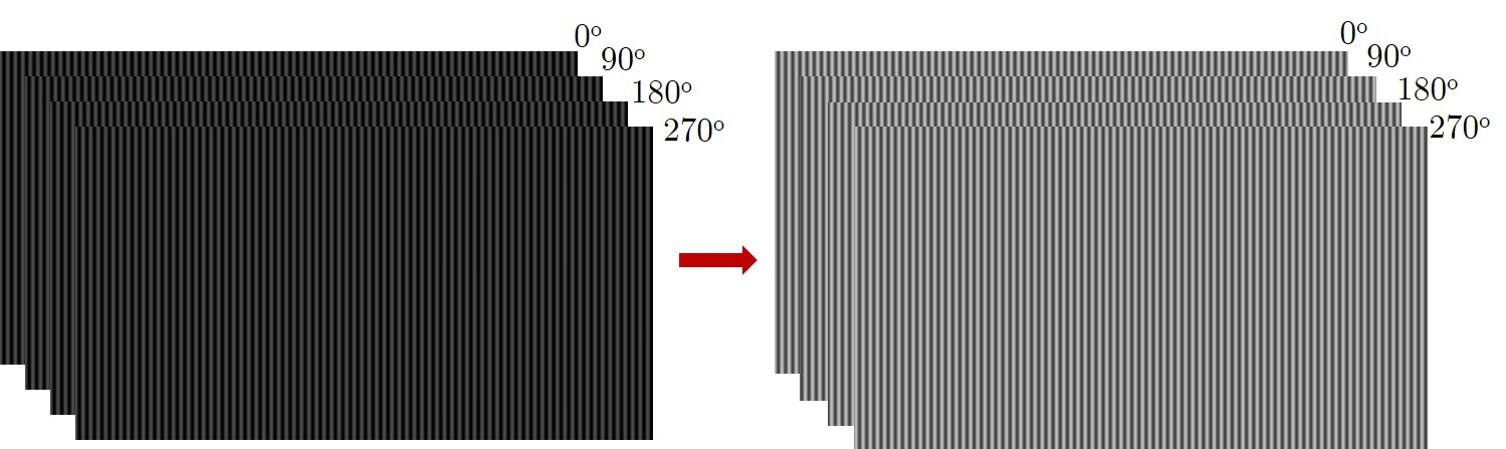
\includegraphics[width=1\textwidth]{figures/fringes.jpg}
	\caption{Fringes before (left) and after biasing (right).}
	\label{fig:fringes}
\end{figure}

Based from the result of linearization, a biasing in the fringes was implemented to get better quality 2D images for the 3D reconstruction.
The obtained polynomial curve was fitted to the original fringe.

A constant was simply added to the sine wave equation but with the other parameters retained resulting to the following modified equation: 

\begin{equation}
fringe_{biased} = I_o(\sin(2\pi f t + n\phi) + 2)
\end{equation}

This constant shifted the intensity of the projected fringes to a higher minimum and maximum that is within the most linearized range of the camera-projector pair. Figure \ref{fig:fringes} shows the image of the original fringe and the change in the intensity level of the fringes upon application of biasing.

Gamma inversion/correction need not be done several times for a particular camera-projector pair once the fringes are biased to fit the linear range. Changes in the form of the polynomial curve for different camera settings were found to only have shifts for the constant part (p5) but the shape of the curve retains. 


\chapter{Vignetting Correction through Background Subtraction}

\section{Vignetting effect of digital imaging systems}

Vignetting effect refers to an apparent nonuniform illumination of light, seen as a gradual fading of image near its periphery \cite{Hecht2007}. 
Although this is the common definition of vignetting which is symmetric in nature \footnote{vignetting is most often referred to as \textit{radial falloff}}, we will refer to all forms of nonuniform illumination of light in digital imaging systems as vignetting in this paper.

Projectors and cameras have their own vignetting properties. 
For cameras, depending on the set aperture size, light is blocked at the opening which causes the vignetting effect \cite{Hecht2007}. 
For projectors, it may depend upon the position and orientation of the projector and even the reflectance property of the screen \cite{Juang2007}. 

Previous works on correction of vignetting effect required using fixed zoom settings for both camera-projector pair \cite{Juang2007}, or fixed lighting conditions \cite{}, dealing with them individually by getting their intrinsic and extrinsic parameters \cite{Goldman2010}. 
In Vergara's thesis \cite{Vergara2010}, vignetting effect of the camera was reduced by setting the camera aperture to the lowest possible size. Although this proved to be a good solution due to its simplicity, it is only limited to the camera and does not extend to correction of vignetting of projector and/or the whole PSP system.

The placement of both projector and camera relative to the object surface in a PSP setup also causes vignetting effect resulting to a wrong depth or height perception of the object upon phase retrieval. The relative placement of the equipment may change from one experiment to another. On-site experiments will also have varying lighting conditions. Thus, repeated calibration may prove to be inefficient and the solutions above may not be appropriate to use. 


\section{Illustrations using a flat white image}
To measure the vignetting effect of the camera, a white image was captured with the camera settings set to an aperture size of f/4 and exposure time to 1/40 seconds. 
Vignetting effect becomes more visible with increasing aperture size \cite{Juang2007}. 
Mesh images of white 
%Thus, with such large aperture size, background subtraction was further implemented to completely remove the vignetting effect. 
%We smoothened first the white background image by taking the mean of its small blocks (4x4 pixels) and the smoothened image is then divided to the original one.

\captionsetup[figure]{width=5in}
\begin{figure}[h!]
%\centering{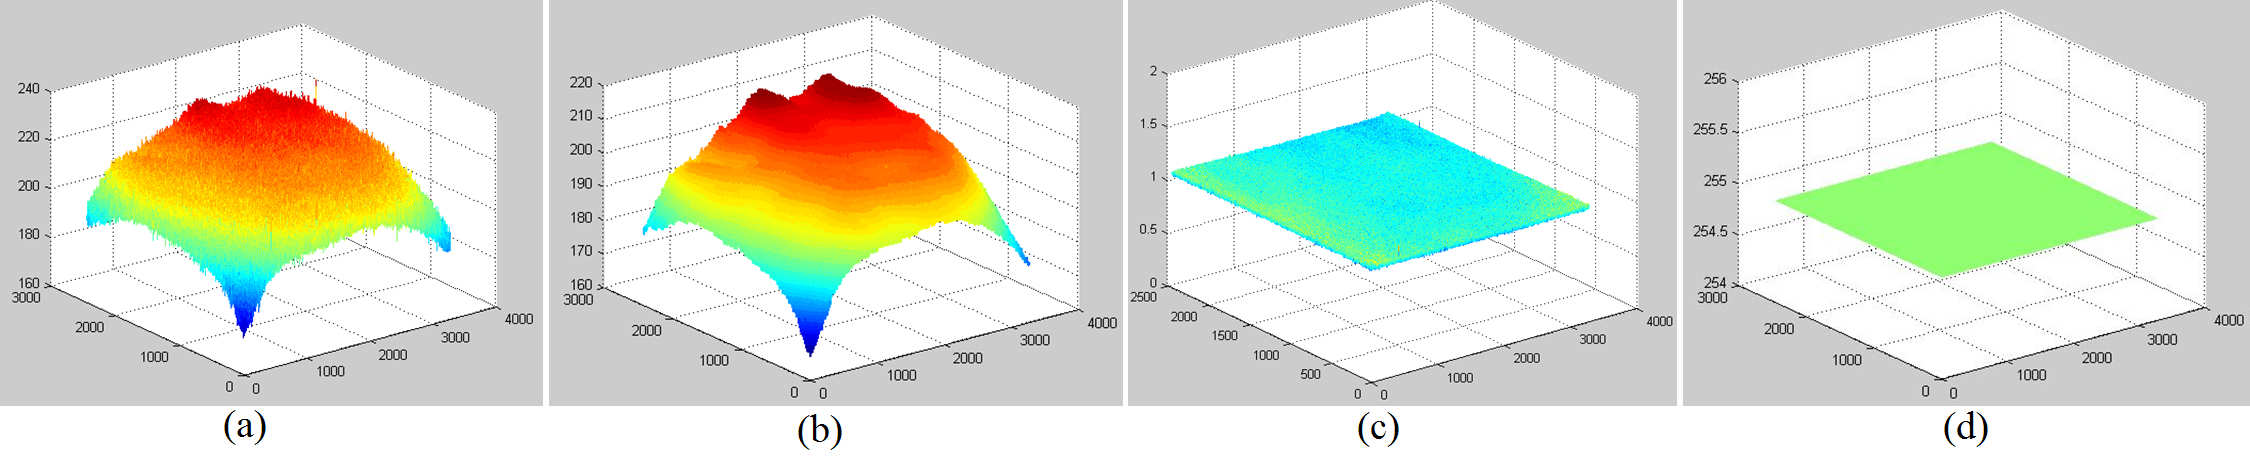
\includegraphics[width=4in]{mesh.jpg}}
\caption{Mesh intensity profiles of the white background (a) output image at f/4 (b) smoothened output image (c) smoothened output image with background subtraction (d) output image at f/22. }
\label{fig:mesh}
\end{figure}





As a comparison, the aperture was also set to f/22, the optimal aperture setting that the camera is capable of, and the exposure time to 2.5 seconds to compensate for the small aperture size. 
Figure \ref{fig:mesh} shows the mesh intensity profiles of the white image. 
%and the processes done to remove the vignetting effect. 
%We see that background subtraction from Figure \ref{fig:mesh}c indeed removed the vignetting effect but still has a small amount of noise. 
%However, the output image captured at f/22 aperture size has no vignetting effects at all and no visible noise. Thus, the f/22 aperture size was chosen for the camera setting.

\section{Correcting vignetting effect on a PSP system}

Depending on the object, two methods for background subtraction may be performed for correcting vignetting effect. These techniques may be applied depending upon the range of height variation of a test object. 

\subsection{Direct Background Subtraction}

For plane/flat surfaces with minimal details of relative uniform depth, we used the resulting phase map itself to serve as the background. 
We took the mean of its small blocks (m x n pixels) and applied bicubic interpolation. The block size was carefully chosen so as not to remove the details.
The interpolated image is then subtracted to the unprocessed phase map. We refer to this process as the Direct Background Subtraction (DBS) method.

\subsection{Reference Background Subtraction}

A different approach was used for objects of nonuniform depth/height. 
DBS may only be used for this type if phase unwrapping is done per region, i.e. nonuniform illumination is less apparent if not observable for a subregion of an image; hence, it will be easier to correct it without deforming the details (modified DBS).

However, this is a tedious and highly time consuming process especially for large images and thus, we disregarded this method. As a resolution, a white image (unto which PSP is also performed) was used as the reference and its unwrapped phase was subsequently subtracted to that of the object's unwrapped phase and we call this the Reference Background Subtraction (RBS) method.

\subsection{3D reconstruction}
Figure \ref{fig:stone} shows the reference and object unwrapped phases of the pebbled wall portion. 
We see a nonuniform phase for the reference's unwrapped phase even if it is supposed to be a flat white image.

\captionsetup[figure]{width=5in}
\begin{figure}[h!]
	\centering
	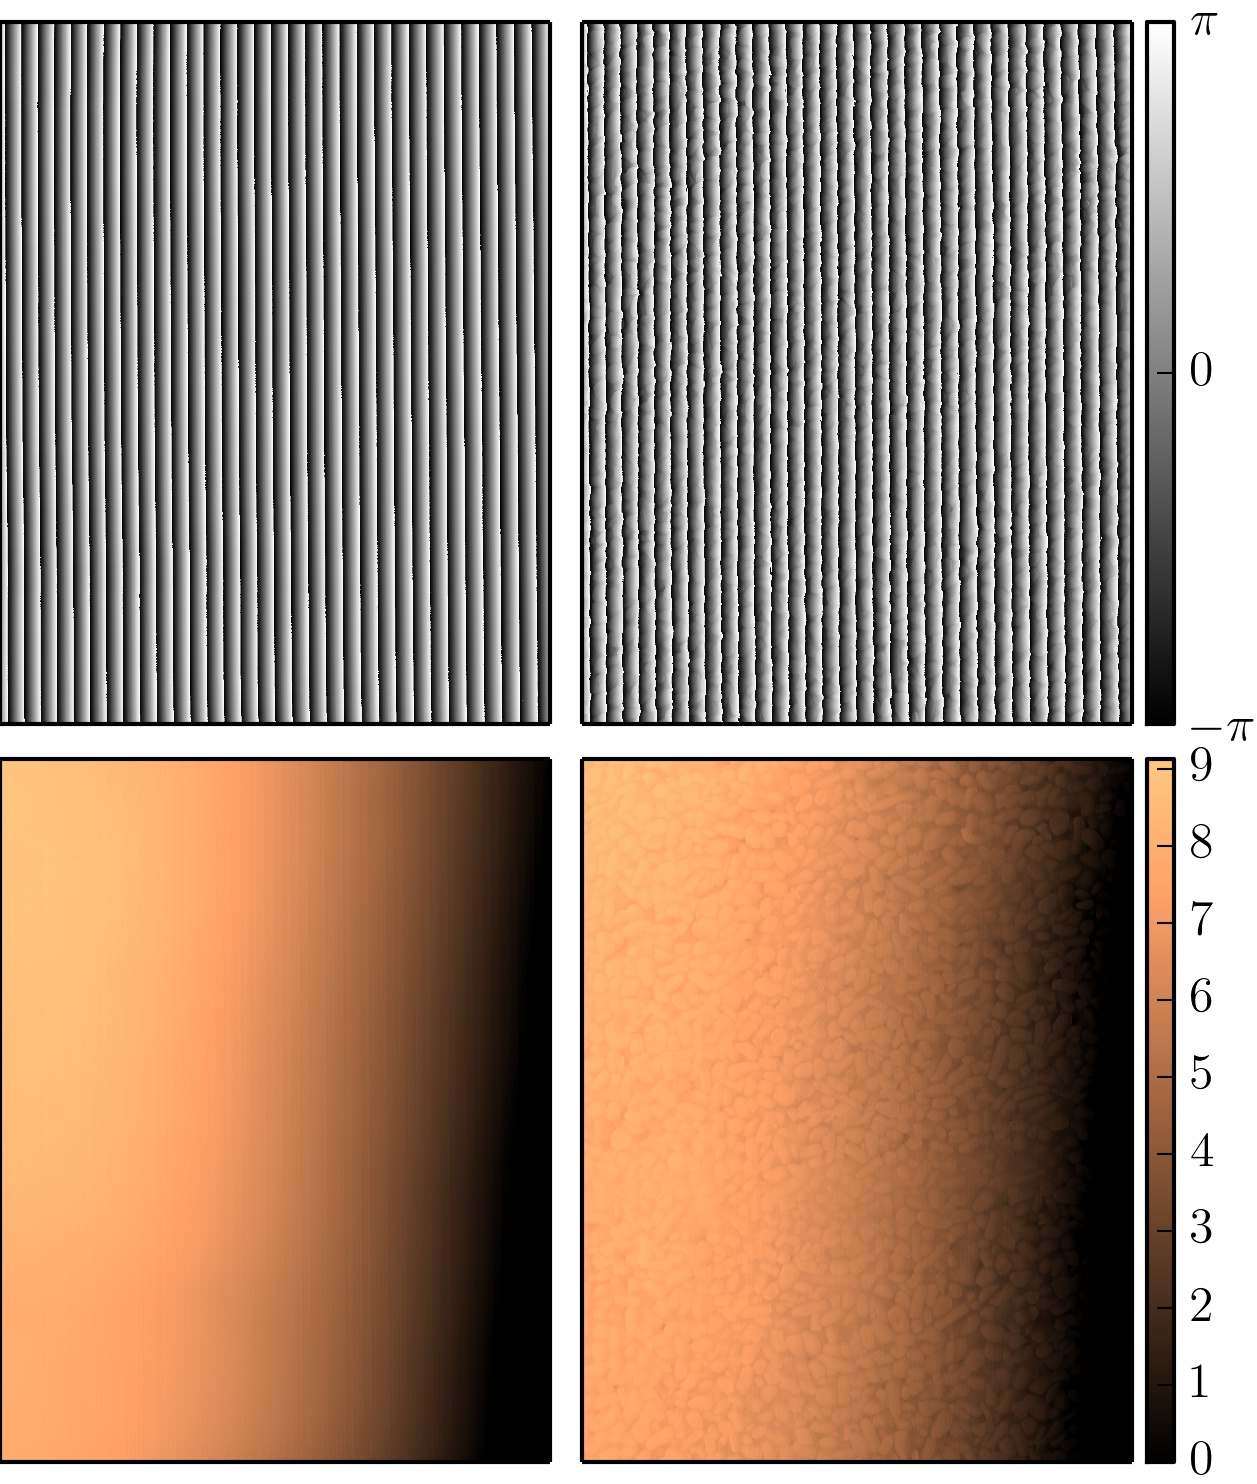
\includegraphics[width=0.62\textwidth]{figures/stone_copper.jpg}
	\caption{Wrapped (top) and unwrapped phase maps of the reference (right) and the pebbled wall (left). The images are displayed in `copper' colormap to match color of the actual object.}
	\label{fig:stone}
\end{figure}

This is an indication of the nonuniform illumination of light which is also seen in the object's unwrapped phase. 
Hence, the details of the pebbled wall are not observable.

RBS and DBS are implemented to the unwrapped phase of the pebbled wall. 
The details of the pebbled wall are now observable but the resulting phase map from using RBS still has an apparent nonuniform intensity while DBS is more uniform. 

\captionsetup[figure]{width=5in}
\begin{figure}[h!t]
	\centering
	\subfigure[]{\includegraphics[width=0.45\textwidth]{figures/stoneRBS.pdf}\label{fig:RBS}}
	\subfigure[]{\includegraphics[width=0.45\textwidth]{figures/stoneDBS.pdf}\label{fig:DBS}}
	\caption{Resulting phase maps after using (a) RBS and (b) DBS.}
	\label{fig:stoneBS}
\end{figure}

Shown in Figure \ref{fig:stonehist} is the histogram distribution of the phase values after application of RBS and DBS. We see that the RBS has a wider distribution of phase values as compared to DBS. The standard deivation of the two were also obtained: RBS = 0.315, DBS = 0.201. Higher standard deviation means a higher distribution of phase values (greater nonuniformity). 


\captionsetup[figure]{width=5in}
\begin{figure}[h!]
	\centering
	\includegraphics[width=0.75\textwidth]{figures/stonehisto.pdf}
	\caption{Histogram distribution of phase values of the pebbled wall after RBS and DBS from Figure~\ref{fig:DBS}.}
	\label{fig:stonehist}
\end{figure}

DBS is better for flat objects with minimal details (depth/height of less than 10 mm). As for RBS, incorrectly placing the reference during the experiment will lead to discrepancies in phase values.

\chapter{FFT Filtering for Removal of Sinusoidal Fringe Artifacts}

\section{Two-Dimensional Fourier Transform}

%Another source of artifact which needed to be resolved are the fringes which remain in the unwrapped phase. 
%A method that can remove this is filtering of the unwanted frequencies in the Fourier domain. 

The Fourier Transform (FT) of a complex signal is the spatial frequency distribution of that signal. The FT of an image f(x,y) is given by

\begin{equation}
F(f_x, f_y) = \iint f(x,y) \exp(-i2\pi(f_xx+f_yy)) dx dy
\end{equation}
where $f_x$ and $f_y$ are the spatial frequencies along x and y, respectively  \cite{Wahl1987}. Calculation for the 2D FT has a very high computational time that an algorithm exploiting its separability and symmetry was introduced. This fast and efficient algorithm is the Fast Fourier Transform (FFT) and it substantially reduces computational time.

From the FFT of an image, observations of the repetitive patterns and  artifacts in the image can be easily done. In some images, these repetitive patterns and artifacts maybe unwanted noise that needed to be remove. However, removing these artifacts may be impossible to do in the image itself without affecting the other details. The FFT then allows us to analyze and process the image in the Fourier domain by removing or enhancing only the desired frequencies \cite{Cad2006}.
\section{Filtering in the frequency domain}

\chapter{3D Reconstructions and Applications on Angono Petroglyph Scale Models}

\input{3Dmodels/angonomodel.tex}
\section{Angono petroglyphs}


\chapter{Summary}



\appendix
\chapter{Quality-Guided Path Unwrapping Algorithm}

As discussed in Section 2.3.2, the general algorithm which was used for phase unwrapping is the \textit{quality-guided path unwrapping algorithm} of Herraez, et al. which has a unique localized unwrapping path \cite{Herraez2002}.

All the figures and algorithms that will be shown in here are excerpts from their paper: ``Fast two-dimensional phase-unwrapping algorithm based on sorting by reliability following a noncontinuous path \cite{Herraez2002}."

The general flow of the algorithm will be illustrated in the following figures containing some numerical examples. Supposed we now have the computed reliability values for each pixel as shown in Fig. (a), an edge's reliability will be computed as the summation of the reliabilities the edge connects in Fig. (b) wherein the ones colored in red are vertically connected edges and colored in green are horizontally connected edges.

Unwrapping path is not defined by the reliability of the pixels but the reliability of the edges. The edges are stored in an array and sorted according to their reliability values. The edges with a higher reliabilities are unwrapped first.

\captionsetup[figure]{width=6in}
\begin{figure}[h!]
	\centering
	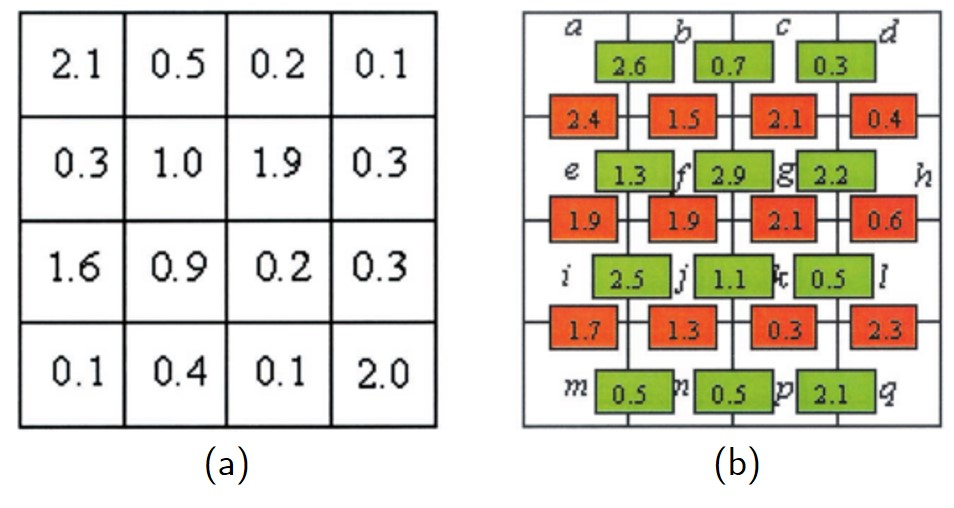
\includegraphics[width=0.7\textwidth]{figures/unwrap1.jpg}
	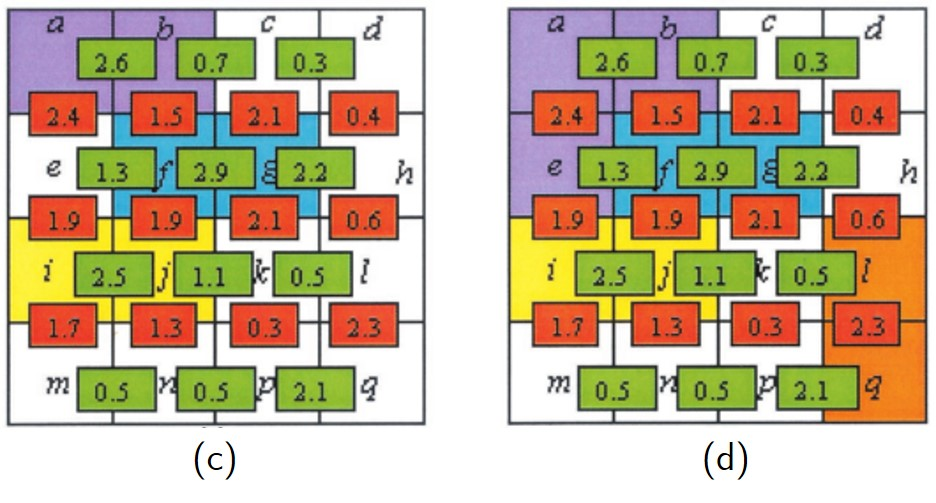
\includegraphics[width=0.7\textwidth]{figures/unwrap2.jpg}
	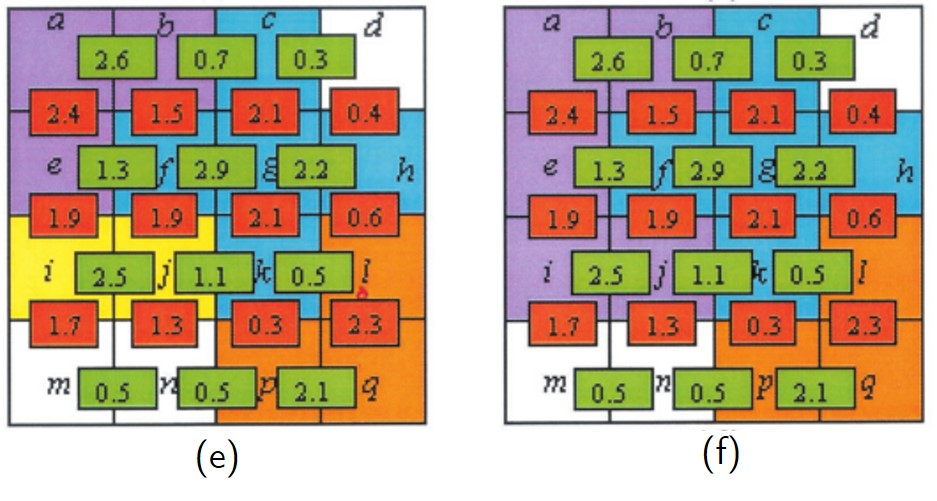
\includegraphics[width=0.7\textwidth]{figures/unwrap3.jpg}
	\caption[Unwrapping path]{Illustration of unwrapping path using numerical examples.}
	\label{fig:unwrap}
\end{figure}

For the unwrapping, pixels are initially considered as not belonging to any group. As seen in Fig. (c), the pixels with the highest reliability value (2.9) are \textit{f} and \textit{g} ($1^{st}$ group), thus they are unwrapped first with respect to each other. Pixels \textit{a} and \textit{b} are unwrapped next ($2^{nd}$ group) followed by pixels \textit{i} and \textit{j} ($3^{rd}$ group).

We see in Fig. (c) and (d) that the fourth highest value for an edge is shared by \textit{a} and \textit{e} and they should be unwrapped with respect to each other. However, \textit{a} is already unwrapped with respect to \textit{b} and has their own group. To unwrap pixel \textit{e}, the 2$\pi$ multiples required to be added/subtracted to unwrap pixel \textit{e} is calculated and added/subtracted to it. Pixels a, b, and e will now have the same group and is colored as one as shown in Fig. (d). 

\captionsetup[figure]{width=6in}
\begin{figure}[h!]
	\centering
	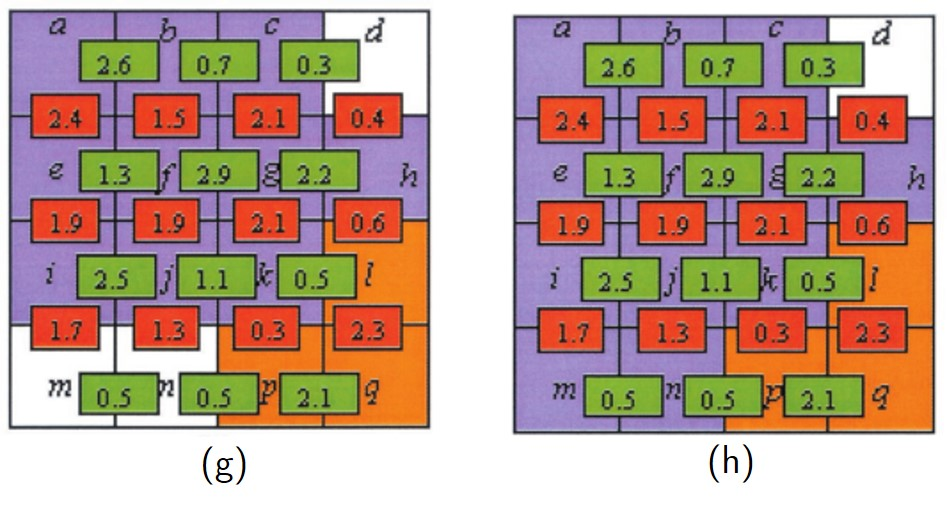
\includegraphics[width=0.7\textwidth]{figures/unwrap4.jpg}
	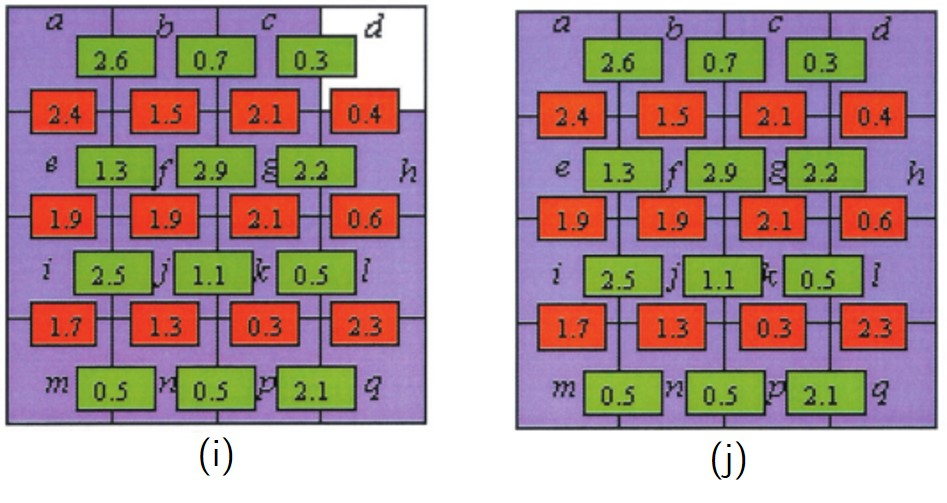
\includegraphics[width=0.7\textwidth]{figures/unwrap5.jpg}
	\caption[Continuation of unwrapping path]{Unwrapping path (\textit{continuation...}).}
	\label{fig:unwrap1}
\end{figure}

Fig. (e) and (f) illustrate the unwrapping of two groups with respect to each other with the first group consisting of pixels \textit{a}, \textit{b}, and \textit{e} and second group having pixels \textit{i} and \textit{j}. They are connected by a vertical edge and they share the next highest reliability value for an edge. Both groups are unwrapped with respect to each other. A pixel that belongs to the smaller group (less number of pixels) is unwrapped first with respect to any pixel in the larger group and the two groups will be joined together and colored as one as shown in Fig. (f). 

The algorithm will then proceed as shown in Fig. \ref{fig:unwrap1} until all pixels are unwrapped.


\chapter{Code Snippets}
%\lstset{caption={\textbf{} Defines vehicle objects and methods}}
\lstinputlisting[language=Python]{PSPphaseUnwrap.py}

%\bibliographystyle{osa}
%\bibliography{library} %% see file: "biblio.bib"
\setlength{\bibitemsep}{\baselineskip}
\printbibliography
\end{document}
%%end of main.tex
